% Generated fragments require trusted human review before compilation.
% This binder never requests shell escape or runs external tools.
\documentclass[11pt]{article}
% Trusted shared apparatus. Requires LuaLaTeX; never use shell escape.
\usepackage{fontspec}
\defaultfontfeatures{Ligatures=TeX}
\IfFontExistsTF{Noto Serif}{\setmainfont{Noto Serif}}{%
  \IfFontExistsTF{DejaVu Serif}{\setmainfont{DejaVu Serif}}{%
    \IfFontExistsTF{Times New Roman}{\setmainfont{Times New Roman}}{%
      \PackageError{gelfand-binder}{No configured Cyrillic serif font installed}{Install Noto Serif or DejaVu Serif, or select an installed Cyrillic font.}%
    }%
  }%
}
\IfFontExistsTF{Noto Sans}{\setsansfont{Noto Sans}}{%
  \IfFontExistsTF{DejaVu Sans}{\setsansfont{DejaVu Sans}}{\setsansfont{Arial}}%
}
\IfFontExistsTF{Noto Sans Mono}{\setmonofont{Noto Sans Mono}}{%
  \IfFontExistsTF{DejaVu Sans Mono}{\setmonofont{DejaVu Sans Mono}}{\setmonofont{Courier New}}%
}
\usepackage[a4paper,margin=22mm]{geometry}
\usepackage{amsmath,amssymb,amsthm,mathtools}
\usepackage{xcolor}
\usepackage{tikz}
\usepackage{tikz-cd}
\usetikzlibrary{arrows.meta,positioning,calc}
\usepackage{hyperref}
\hypersetup{unicode=true,colorlinks=true,linkcolor=blue,pdftitle={Gelfand transcription binder}}
\newtheorem{theorem}{Theorem}
\newtheorem{lemma}{Lemma}
\newtheorem{proposition}{Proposition}
\newtheorem{corollary}{Corollary}
\theoremstyle{definition}
\newtheorem{definition}{Definition}
\newtheorem{example}{Example}
\theoremstyle{remark}
\newtheorem{remark}{Remark}
\setlength{\parindent}{0pt}
\setlength{\parskip}{0.55em}
\setlength{\emergencystretch}{3em}
\newcommand{\SourcePage}[2]{%
  \clearpage\phantomsection\label{#1:source-page}%
  \addcontentsline{toc}{subsection}{#1}%
  {\small\sffamily\color{blue!60!black}Source scan frame: #1; visible page/leaf label: #2}\par\medskip%
}
\newcommand{\Unclear}[3]{%
  \begingroup\color{orange!70!black}%
  [Unresolved reading #1/#2: #3]\endgroup%
}
\newcommand{\Incomplete}[3]{%
  \par\begingroup\color{red!65!black}\textbf{Incomplete #1/#2:} #3\endgroup\par%
}
\newcommand{\SourceFigure}[3]{%
  \par\begingroup\color{blue!60!black}\textbf{\hyperref[#1:source-page]{Source figure #1/#2}:} #3%
  \par\textit{Consult the authoritative scan at this locator.}\endgroup\par%
}



% Reader layout only. Original diplomatic text is retained verbatim.
\setlength{\parskip}{0.35em}
\setlength{\emergencystretch}{4em}
\renewcommand{\SourcePage}[2]{%
  \par\addvspace{1em}\phantomsection\label{#1:source-page}%
  \addcontentsline{toc}{subsection}{#1}%
  {\footnotesize\sffamily\color{blue!55!black}#1%
    \def\givenlabel{#2}\def\nolabel{unlabelled}%
    \ifx\givenlabel\nolabel\else\quad[номер в источнике: #2]\fi
  }\par\nobreak\smallskip%
}
\renewcommand{\Unclear}[3]{%
  \begingroup\color{orange!65!black}%
  \ifmmode\text{[неясно: #3]}\else[неясно: #3]\fi\endgroup%
}
\renewcommand{\Incomplete}[3]{%
  \par\begingroup\color{red!60!black}\textbf{Неразобранный фрагмент:} #3%
  \endgroup\par%
}
\renewcommand{\SourceFigure}[3]{%
  \par\begingroup\color{blue!55!black}\textbf{Рисунок:} #3%
  \par{\small\textit{Исходный рисунок: \hyperref[#1:source-page]{#1}, #2.}}%
  \endgroup\par%
}
\hypersetup{pdftitle={Семинар И. М. Гельфанда. Дипломатическая транскрипция},pdfauthor={},pdfsubject={Русское рабочее издание с отмеченными сомнительными чтениями}}

\usepackage[normalem]{ulem}
\usepackage{newunicodechar}
\usepackage{adjustbox}
\newfontfamily\SourceSymbolFont{Segoe UI Symbol}
\newfontfamily\SourceCJKFont{MS Gothic}
\let\DiplomaticMathUnderline\underline
\renewcommand{\underline}[1]{\ifmmode\DiplomaticMathUnderline{#1}\else\uline{#1}\fi}
\newunicodechar{→}{\ifmmode\text{{\SourceSymbolFont\char"2192}}\else{\SourceSymbolFont\char"2192}\fi}
\newunicodechar{⇒}{\ifmmode\text{{\SourceSymbolFont\char"21D2}}\else{\SourceSymbolFont\char"21D2}\fi}
\newunicodechar{∀}{\ifmmode\text{{\SourceSymbolFont\char"2200}}\else{\SourceSymbolFont\char"2200}\fi}
\newunicodechar{∂}{\ifmmode\text{{\SourceSymbolFont\char"2202}}\else{\SourceSymbolFont\char"2202}\fi}
\newunicodechar{∈}{\ifmmode\text{{\SourceSymbolFont\char"2208}}\else{\SourceSymbolFont\char"2208}\fi}
\newunicodechar{∌}{\ifmmode\text{{\SourceSymbolFont\char"220C}}\else{\SourceSymbolFont\char"220C}\fi}
\newunicodechar{√}{\ifmmode\text{{\SourceSymbolFont\char"221A}}\else{\SourceSymbolFont\char"221A}\fi}
\newunicodechar{∞}{\ifmmode\text{{\SourceSymbolFont\char"221E}}\else{\SourceSymbolFont\char"221E}\fi}
\newunicodechar{∧}{\ifmmode\text{{\SourceSymbolFont\char"2227}}\else{\SourceSymbolFont\char"2227}\fi}
\newunicodechar{∩}{\ifmmode\text{{\SourceSymbolFont\char"2229}}\else{\SourceSymbolFont\char"2229}\fi}
\newunicodechar{∪}{\ifmmode\text{{\SourceSymbolFont\char"222A}}\else{\SourceSymbolFont\char"222A}\fi}
\newunicodechar{∫}{\ifmmode\text{{\SourceSymbolFont\char"222B}}\else{\SourceSymbolFont\char"222B}\fi}
\newunicodechar{∴}{\ifmmode\text{{\SourceSymbolFont\char"2234}}\else{\SourceSymbolFont\char"2234}\fi}
\newunicodechar{∼}{\ifmmode\text{{\SourceSymbolFont\char"223C}}\else{\SourceSymbolFont\char"223C}\fi}
\newunicodechar{≈}{\ifmmode\text{{\SourceSymbolFont\char"2248}}\else{\SourceSymbolFont\char"2248}\fi}
\newunicodechar{≠}{\ifmmode\text{{\SourceSymbolFont\char"2260}}\else{\SourceSymbolFont\char"2260}\fi}
\newunicodechar{≤}{\ifmmode\text{{\SourceSymbolFont\char"2264}}\else{\SourceSymbolFont\char"2264}\fi}
\newunicodechar{≥}{\ifmmode\text{{\SourceSymbolFont\char"2265}}\else{\SourceSymbolFont\char"2265}\fi}
\newunicodechar{⊕}{\ifmmode\text{{\SourceSymbolFont\char"2295}}\else{\SourceSymbolFont\char"2295}\fi}
\newunicodechar{⊗}{\ifmmode\text{{\SourceSymbolFont\char"2297}}\else{\SourceSymbolFont\char"2297}\fi}
\newunicodechar{①}{\ifmmode\text{{\SourceSymbolFont\char"2460}}\else{\SourceSymbolFont\char"2460}\fi}
\newunicodechar{②}{\ifmmode\text{{\SourceSymbolFont\char"2461}}\else{\SourceSymbolFont\char"2461}\fi}
\newunicodechar{③}{\ifmmode\text{{\SourceSymbolFont\char"2462}}\else{\SourceSymbolFont\char"2462}\fi}
\newunicodechar{④}{\ifmmode\text{{\SourceSymbolFont\char"2463}}\else{\SourceSymbolFont\char"2463}\fi}
\newunicodechar{Ⓗ}{\ifmmode\text{{\SourceSymbolFont\char"24BD}}\else{\SourceSymbolFont\char"24BD}\fi}
\newunicodechar{〃}{\ifmmode\text{{\SourceCJKFont\char"3003}}\else{\SourceCJKFont\char"3003}\fi}


% Reader revision 3. Annotation wording and candidates remain unchanged.
\setmainfont{NotoSerif-Regular.ttf}[Path=C:/Windows/Fonts/,ItalicFont=NotoSerif-Italic.ttf,BoldFont=NotoSerif-Bold.ttf,BoldItalicFont=NotoSerif-BoldItalic.ttf]
\usetikzlibrary{shapes.geometric,decorations.pathreplacing,decorations.markings,patterns,fit}
\newsavebox{\ReaderAnnotationBox}
\newcommand{\ReaderAnnotation}[1]{%
  \sbox{\ReaderAnnotationBox}{[неясно: #1]}%
  \ifdim\wd\ReaderAnnotationBox>.70\linewidth
    \parbox[t]{.70\linewidth}{\raggedright[неясно: #1]}%
  \else\usebox{\ReaderAnnotationBox}\fi%
}
\ExplSyntaxOn
\cs_new_protected:Npn \reader_unclear_candidate:n #1
 {
  \tl_set:Nx \l_tmpa_tl { \tl_to_str:n {#1} }
  % Text explicitly guarded inside a mathematical candidate remains math-safe.
  \regex_replace_all:nnN { \\(?:text|textrm|textnormal|textbf|operatorname)\s*\{[^{}]*\} } { } \l_tmpa_tl
  \regex_match:nVTF { [\x{0400}-\x{052F}] | \$ } \l_tmpa_tl
   { \ifmmode \text{\ReaderAnnotation{#1}} \else \ReaderAnnotation{#1} \fi }
   {
    \ifmmode
      [\text{неясно:~}#1]
    \else
      \regex_match:nVTF { [_^] | \\ } \l_tmpa_tl
       { \ensuremath{[\text{неясно:~}#1]} }
       { \ReaderAnnotation{#1} }
    \fi
   }
 }
\RenewDocumentCommand \Unclear { m m m }
 { \begingroup\color{orange!65!black}\reader_unclear_candidate:n{#3}\endgroup }
\ExplSyntaxOff
\newsavebox{\ReaderIncompleteBox}
\newcommand{\ReaderIncompleteNote}[1]{%
 \sbox{\ReaderIncompleteBox}{\textbf{Неразобранный фрагмент:} #1}%
 \ifdim\wd\ReaderIncompleteBox>.70\linewidth
  \parbox[t]{.70\linewidth}{\raggedright\textbf{Неразобранный фрагмент:} #1}%
 \else\usebox{\ReaderIncompleteBox}\fi%
}
\renewcommand{\Incomplete}[3]{%
 \ifmmode\text{\color{red!60!black}\ReaderIncompleteNote{#3}}%
 \else\leavevmode\begingroup\color{red!60!black}\ReaderIncompleteNote{#3}\endgroup\fi%
}
% Ragged right avoids stretching long untranslated abbreviations into margins.
\AtBeginDocument{\raggedright}
\newunicodechar{А}{\ifmmode\text{\char"410\relax}\else\char"410\relax\fi}
\newunicodechar{Б}{\ifmmode\text{\char"411\relax}\else\char"411\relax\fi}
\newunicodechar{В}{\ifmmode\text{\char"412\relax}\else\char"412\relax\fi}
\newunicodechar{Г}{\ifmmode\text{\char"413\relax}\else\char"413\relax\fi}
\newunicodechar{Д}{\ifmmode\text{\char"414\relax}\else\char"414\relax\fi}
\newunicodechar{Е}{\ifmmode\text{\char"415\relax}\else\char"415\relax\fi}
\newunicodechar{Ж}{\ifmmode\text{\char"416\relax}\else\char"416\relax\fi}
\newunicodechar{З}{\ifmmode\text{\char"417\relax}\else\char"417\relax\fi}
\newunicodechar{И}{\ifmmode\text{\char"418\relax}\else\char"418\relax\fi}
\newunicodechar{Й}{\ifmmode\text{\char"419\relax}\else\char"419\relax\fi}
\newunicodechar{К}{\ifmmode\text{\char"41A\relax}\else\char"41A\relax\fi}
\newunicodechar{Л}{\ifmmode\text{\char"41B\relax}\else\char"41B\relax\fi}
\newunicodechar{М}{\ifmmode\text{\char"41C\relax}\else\char"41C\relax\fi}
\newunicodechar{Н}{\ifmmode\text{\char"41D\relax}\else\char"41D\relax\fi}
\newunicodechar{О}{\ifmmode\text{\char"41E\relax}\else\char"41E\relax\fi}
\newunicodechar{П}{\ifmmode\text{\char"41F\relax}\else\char"41F\relax\fi}
\newunicodechar{Р}{\ifmmode\text{\char"420\relax}\else\char"420\relax\fi}
\newunicodechar{С}{\ifmmode\text{\char"421\relax}\else\char"421\relax\fi}
\newunicodechar{Т}{\ifmmode\text{\char"422\relax}\else\char"422\relax\fi}
\newunicodechar{У}{\ifmmode\text{\char"423\relax}\else\char"423\relax\fi}
\newunicodechar{Ф}{\ifmmode\text{\char"424\relax}\else\char"424\relax\fi}
\newunicodechar{Х}{\ifmmode\text{\char"425\relax}\else\char"425\relax\fi}
\newunicodechar{Ц}{\ifmmode\text{\char"426\relax}\else\char"426\relax\fi}
\newunicodechar{Ч}{\ifmmode\text{\char"427\relax}\else\char"427\relax\fi}
\newunicodechar{Ш}{\ifmmode\text{\char"428\relax}\else\char"428\relax\fi}
\newunicodechar{Щ}{\ifmmode\text{\char"429\relax}\else\char"429\relax\fi}
\newunicodechar{Ъ}{\ifmmode\text{\char"42A\relax}\else\char"42A\relax\fi}
\newunicodechar{Ы}{\ifmmode\text{\char"42B\relax}\else\char"42B\relax\fi}
\newunicodechar{Ь}{\ifmmode\text{\char"42C\relax}\else\char"42C\relax\fi}
\newunicodechar{Э}{\ifmmode\text{\char"42D\relax}\else\char"42D\relax\fi}
\newunicodechar{Ю}{\ifmmode\text{\char"42E\relax}\else\char"42E\relax\fi}
\newunicodechar{Я}{\ifmmode\text{\char"42F\relax}\else\char"42F\relax\fi}
\newunicodechar{а}{\ifmmode\text{\char"430\relax}\else\char"430\relax\fi}
\newunicodechar{б}{\ifmmode\text{\char"431\relax}\else\char"431\relax\fi}
\newunicodechar{в}{\ifmmode\text{\char"432\relax}\else\char"432\relax\fi}
\newunicodechar{г}{\ifmmode\text{\char"433\relax}\else\char"433\relax\fi}
\newunicodechar{д}{\ifmmode\text{\char"434\relax}\else\char"434\relax\fi}
\newunicodechar{е}{\ifmmode\text{\char"435\relax}\else\char"435\relax\fi}
\newunicodechar{ж}{\ifmmode\text{\char"436\relax}\else\char"436\relax\fi}
\newunicodechar{з}{\ifmmode\text{\char"437\relax}\else\char"437\relax\fi}
\newunicodechar{и}{\ifmmode\text{\char"438\relax}\else\char"438\relax\fi}
\newunicodechar{й}{\ifmmode\text{\char"439\relax}\else\char"439\relax\fi}
\newunicodechar{к}{\ifmmode\text{\char"43A\relax}\else\char"43A\relax\fi}
\newunicodechar{л}{\ifmmode\text{\char"43B\relax}\else\char"43B\relax\fi}
\newunicodechar{м}{\ifmmode\text{\char"43C\relax}\else\char"43C\relax\fi}
\newunicodechar{н}{\ifmmode\text{\char"43D\relax}\else\char"43D\relax\fi}
\newunicodechar{о}{\ifmmode\text{\char"43E\relax}\else\char"43E\relax\fi}
\newunicodechar{п}{\ifmmode\text{\char"43F\relax}\else\char"43F\relax\fi}
\newunicodechar{р}{\ifmmode\text{\char"440\relax}\else\char"440\relax\fi}
\newunicodechar{с}{\ifmmode\text{\char"441\relax}\else\char"441\relax\fi}
\newunicodechar{т}{\ifmmode\text{\char"442\relax}\else\char"442\relax\fi}
\newunicodechar{у}{\ifmmode\text{\char"443\relax}\else\char"443\relax\fi}
\newunicodechar{ф}{\ifmmode\text{\char"444\relax}\else\char"444\relax\fi}
\newunicodechar{х}{\ifmmode\text{\char"445\relax}\else\char"445\relax\fi}
\newunicodechar{ц}{\ifmmode\text{\char"446\relax}\else\char"446\relax\fi}
\newunicodechar{ч}{\ifmmode\text{\char"447\relax}\else\char"447\relax\fi}
\newunicodechar{ш}{\ifmmode\text{\char"448\relax}\else\char"448\relax\fi}
\newunicodechar{щ}{\ifmmode\text{\char"449\relax}\else\char"449\relax\fi}
\newunicodechar{ъ}{\ifmmode\text{\char"44A\relax}\else\char"44A\relax\fi}
\newunicodechar{ы}{\ifmmode\text{\char"44B\relax}\else\char"44B\relax\fi}
\newunicodechar{ь}{\ifmmode\text{\char"44C\relax}\else\char"44C\relax\fi}
\newunicodechar{э}{\ifmmode\text{\char"44D\relax}\else\char"44D\relax\fi}
\newunicodechar{ю}{\ifmmode\text{\char"44E\relax}\else\char"44E\relax\fi}
\newunicodechar{я}{\ifmmode\text{\char"44F\relax}\else\char"44F\relax\fi}
\newunicodechar{Ё}{\ifmmode\text{\char"401\relax}\else\char"401\relax\fi}
\newunicodechar{ё}{\ifmmode\text{\char"451\relax}\else\char"451\relax\fi}

\newunicodechar{æ}{\ifmmode\text{\char"E6\relax}\else\char"E6\relax\fi}
\newunicodechar{−}{\ifmmode\mathbin{\text{\SourceSymbolFont\char"2212\relax}}\else{\SourceSymbolFont\char"2212\relax}\fi}

\begin{document}
\begin{center}
{\Large Семинар И. М. Гельфанда}\par\medskip
{\LARGE Дипломатическая транскрипция}\par\bigskip
{\large Рабочее русское издание}\par\medskip
{\large Том 21 из 34. Архивная глава 021}\par\bigskip
Кадры GELFAND-P001001 -- GELFAND-P001025\par

\end{center}
\medskip
Сокращения, отменённые записи и сомнительные чтения сохранены.
Неразобранные фрагменты отмечены в тексте. Математические утверждения
источника переданы без молчаливых исправлений.

Это рабочее издание: сверка с рукописью продолжается. В текущем комплекте
учтены 1503 из 1527 кадров; 24 кадра пока представлены явными указателями
отсутствующего возврата. Полный журнал чтений и происхождения данных
сохранён в основном рабочем переплёте.

Границы кадров показаны небольшими синими указателями; печатный текст
продолжается без обязательного разрыва страницы после каждого кадра.
\bigskip\hrule\bigskip
\SourcePage{GELFAND-P001001}{unlabelled}
% Review coordinates: original pixels (x0,y0,x1,y1), origin at upper left.
% Enlargements are nearest-neighbour crops, not new source resolution.
% Reviewed top: bbox=(80,1040,1850,1620); scale=1.5x.
% Reviewed middle: bbox=(120,1580,1850,2460); scale=1.5x.
% Reviewed bottom: bbox=(120,2410,1920,3370); scale=1.5x.
% Reviewed collaborator: bbox=(1280,1260,1590,1390); scale=3x.
% Reviewed bibliography: bbox=(285,3220,1480,3345); scale=3x.
% Reviewed equation-two: bbox=(465,2100,875,2245); scale=4x.
% Reviewed momentum-sign: bbox=(900,1715,1505,1860); scale=3x.
% Оригинал 2408 x 3448. Координаты областей в журнале: от левого верхнего угла, в пикселях.
\begin{center}— . —\end{center}
\underline{\underline{8/II-82г.}}\qquad \underline{Сем. Гельфанда}.

\underline{\underline{Müller Werner}}.

\underline{Lattice gravity}. (раб. с Cheeger и Schräder)

1) Рассм. 1-мерн. мех. систему с гамильтонианом:
\begin{equation*}
H(p,q)=+\frac{p^2}{2m}+V(q) \tag{1}
\end{equation*}
\begin{equation*}
q\to Q,\quad p\to P\qquad \text{операторы в }L^2(\mathbb R)
\end{equation*}
\begin{equation*}
Qf(x)=xf(x),\qquad Pf(x)=i\hbar\frac{d}{dx}f(x)
\end{equation*}
\Unclear{GELFAND-P001001}{momentum-sign}{[В источнике: $i\hbar$, без минуса.]}
\begin{equation*}
H(p,q)\to\widehat H
\end{equation*}
Рассм. ур-е Шрёдингера
\begin{equation*}
i\frac{\partial}{\partial t}=\hbar^{-1}\widehat H f \tag{2}
\end{equation*}
\Unclear{GELFAND-P001001}{equation-two}{[Слева записано $i\frac{\partial}{\partial t}$; $f$ имеется только справа.]}
зад. эволюцию:
\begin{equation*}
f(x,t)=e^{-i\frac{t}{\hbar}\widehat H}f(x,0) \tag{3}
\end{equation*}
Вер. перехода из $x$ в $x'$ за время [вставлено сверху: от $t_0$ до] $t$ по Фейнману
\begin{equation*}
\langle x'\mid e^{-i\frac{t}{\hbar}\widehat H}\mid x\rangle
=\int_{\substack{\text{по всем путям }x\\x(0)=x,\ x(t)=x'}}
e^{-iS[x]}\prod_{\tau}\frac{dx(\tau)}{2\pi} \tag{4}
\end{equation*}
\begin{equation*}
S[x]=\int_0^t[\dot x^2(\tau)-V(x(\tau))]d\tau \tag{5}
\end{equation*}
\Unclear{GELFAND-P001001}{action-normalization}{[В (4): $e^{-iS[x]}$; в (5): $\dot x^2(\tau)$.]}
(см. посл. глава кн. \Unclear{GELFAND-P001001}{bibliography}{Коноплевой / Коноплёвой} и Попова)

\SourcePage{GELFAND-P001002}{4}
% Review coordinates: original pixels (x0,y0,x1,y1), origin at upper left.
% Enlargements are nearest-neighbour crops, not new source resolution.
% Reviewed top: bbox=(280,0,2310,975); scale=1.5x.
% Reviewed middle: bbox=(270,945,2260,1900); scale=1.5x.
% Reviewed lower: bbox=(265,1830,2315,2690); scale=1.5x.
% Reviewed bottom: bbox=(275,2670,2408,3448); scale=1.5x.
% Reviewed semigroup-exponent: bbox=(730,565,1035,675); scale=5x.
% Reviewed path-integrand: bbox=(1410,530,1730,665); scale=4x.
% Reviewed lorentz-cancellation: bbox=(575,1120,697,1205); scale=5x.
% Reviewed action-cancellation: bbox=(823,1600,1110,1730); scale=4x.
% Reviewed divergence: bbox=(990,2060,2295,2178); scale=3x.
% Reviewed volume-coefficient: bbox=(1090,2480,1390,2605); scale=5x.
% Reviewed measure-exponent: bbox=(1250,2800,1400,2910); scale=5x.
% Reviewed bottom-cancellation: bbox=(300,3185,430,3305); scale=5x.
% Reviewed coefficient-symbol: bbox=(955,2490,1110,2600); scale=6x.
% Reviewed divergence-cancellation: bbox=(1900,2060,2280,2178); scale=5x.
% Reviewed problem-line: bbox=(485,2225,2365,2420); scale=2x.
или: вместо $t$ вставить $t-t_0$

\hspace{2em}вместо $0$ — '' — $t_0$

\underline{М. Кас} придал нек-рый смысл инт. (4) с заменой $i\to1$
\begin{equation*}
\hbar\frac{\partial f}{\partial t}=\widehat H f, \tag{6}
\end{equation*}
тогда
\begin{equation*}
\langle x'\mid e^{-\frac{t}{\hbar}H x}\mid x\rangle
=\int_{\substack{\text{по всем путям}\\x:\,x(0)=x\\x(t)=x'}}
e^{-\int_0^t x(\tau)d\tau}\,dW(x) \tag{7}
\end{equation*}
[Стрелка к $dW(x)$: мера Винера.]
\Unclear{GELFAND-P001002}{semigroup-exponent}{[В показателе слева после $H$ — $x$; возможное чтение $H_x$.]}
\Unclear{GELFAND-P001002}{heat-kernel}{[В (6) справа $+\widehat Hf$; в (7) под интегралом в показателе $x(\tau)$.]}

2) \underline{Гравитация}.
\begin{equation*}
i\mapsto1\qquad\rightsquigarrow
\end{equation*}
[Зачёркнуто: \Unclear{GELFAND-P001002}{lorentz-cancellation}{неразборчиво; возможно «для»}.]
лоренц. метрика $\longmapsto$ риманова метрика.

$M$ — компактное $C^\infty$-мн-зие
\begin{equation*}
\mathcal M=\{\text{пр-во всех рим. метрик на }M\}
\end{equation*}
\begin{equation*}
G=\operatorname{Diff}(M)\quad\text{— калибров. группа.}
\end{equation*}
Действие [зачёркнуто: \Unclear{GELFAND-P001002}{action-cancellation}{неразборчиво; возможно «Эйн…»}; вставлено ниже: Гильберта (– Эйнштейна)]:
\begin{equation*}
S[g]=\lambda\int_M R\,d\operatorname{vol},\qquad
R\text{ — скалярная кривизна} \tag{8}
\end{equation*}
(нетривиально: Эйнштейн считал, что действия нет)

— в $R$ входят 2-е произв. $\Rightarrow$ ур-е \underline{a priori} 4-го порядка

Но локально есть \underline{нековар. добавок} диверг. вида,
[зачёркнуто: \Unclear{GELFAND-P001002}{divergence-cancellation}{«не влияющий» / «не меняющий»}],
не меняющий $S$.

\underline{Задача (И.М.Г.)} Найти все комб. кривизн, где получ. ур-е меньшего порядка.

\underline{«Ответ»}: Эйнштейн и классы Понтрягина. \underline{Действие}:
\begin{equation*}
\int_{\mathcal M/G}e^{-S[g]-\text{[знак]}\operatorname{Vol}(M,g)}d\mu(g) \tag{9}
\end{equation*}
\Unclear{GELFAND-P001002}{volume-coefficient}{[Коэффициент перед $\operatorname{Vol}(M,g)$: $\kappa$ / ϰ / æ.]}

\underline{Формально}:
\begin{equation*}
d\mu(g)=\prod_{x\in M}\det g(x)^{5/2}\prod_{\mu\leq\nu}dg_{\mu\nu}(x) \tag{10}
\end{equation*}
\Unclear{GELFAND-P001002}{measure-exponent}{[Показатель в источнике: $5/2$, без минуса.]}
(Фаддеев – Попов)

Решёточная аппроксимация.

[Слева зачёркнут номер: \Unclear{GELFAND-P001002}{bottom-cancellation}{(11)?}.]
\begin{equation*}
P^n\subset\mathbb R^N\qquad
P^n\underset{\varphi}{\longrightarrow}M\quad\text{триангуляция}
\end{equation*}
[Черта от $P^n$ к подписи:] кусочно линейное подмн-зие

\SourcePage{GELFAND-P001003}{unlabelled}
% Review coordinates: original pixels (x0,y0,x1,y1), origin at upper left.
% Enlargements are nearest-neighbour crops, not new source resolution.
% Reviewed top: bbox=(120,0,1880,750); scale=1.5x.
% Reviewed middle: bbox=(105,750,1720,1840); scale=1.5x.
% Reviewed lower: bbox=(95,1840,2210,2900); scale=1.5x.
% Reviewed bottom: bbox=(80,2830,2408,3448); scale=1.5x.
% Reviewed polyhedron-sphere: bbox=(150,285,1250,550); scale=3x.
% Reviewed skinny-simplex: bbox=(1145,2395,1900,2575); scale=3x.
% Reviewed midpoint-subdivision: bbox=(825,2620,1085,2815); scale=4x.
% Reviewed subdivision-text: bbox=(330,2540,1170,2695); scale=3x.
% Reviewed smooth-reference: bbox=(340,2785,2110,2940); scale=2x.
% Reviewed formula-eighteen-left: bbox=(490,3160,1415,3448); scale=3x.
% Reviewed formula-eighteen-right: bbox=(1380,3205,2408,3448); scale=3x.
% Reviewed formula-note: bbox=(1970,3010,2230,3260); scale=4x.
% Reviewed skinny-caption: bbox=(1250,2460,1700,2560); scale=5x.
% formula-note crop additionally viewed rotated 47 degrees clockwise.
Метрика на $M$ индуцирует кусочно-лин. метр. на $P$.
\begin{equation*}
(P,\ell),\qquad \ell:P^{(1)}\to\mathbb R_+
\end{equation*}
(симп. $\rightsquigarrow$ его длина)

(11)
\SourceFigure{GELFAND-P001003}{polyhedron-sphere}{Слева многогранник с подписью $P$, рядом с верхним левым ребром $\sigma^1$; имеются сплошные и пунктирные рёбра. Стрелка вправо с $\varphi$ под ней ведёт к изображению сферы, подписанной $M=S^2$, с меридианами, экватором и утолщённым участком слева. Точное соединение пунктирных рёбер и утолщённых дуг требует сверки с оригиналом.}

\underline{Дискр. версия $\displaystyle\int_M R\,d\operatorname{vol}$}.
\begin{equation*}
P^n\longrightarrow M\qquad\text{триангуляция} \tag{12}
\end{equation*}
\begin{equation*}
\sigma^{n-2}\subset P^n
\end{equation*}
$\delta(\sigma^{n-2})$ — угловой дефект $\sigma^{n-2}$
\begin{equation*}
\sigma^n\supset\sigma^{n-2}
\end{equation*}
$[\sigma^{n-2},\sigma^n]$ — диэдральный угол
\begin{equation*}
\delta(\sigma^{n-2})=2\pi-\sum_{\sigma^n\supset\sigma^{n-2}}[\sigma^{n-2},\sigma^n] \tag{13}
\end{equation*}
\begin{equation*}
R(P)=\sum_{\sigma^{n-2}\subset P}\delta(\sigma^{n-2})\operatorname{vol}(\sigma^{n-2}) \tag{14}
\end{equation*}
(Regge)

$P_n$ — послед. триангуляций, $P_n\to M$
\begin{equation*}
\operatorname{mesh}(P_n)\underset{n\to\infty}{\longrightarrow}0 \tag{15}
\end{equation*}
\begin{equation*}
\underline{\text{Th.}}\quad\underline{\text{Тогда}}\quad
R(P_n)\underset{n\to\infty}{\longrightarrow}\int_M R\,d\operatorname{vol} \tag{16}
\end{equation*}
Пока неясно, сходятся ли ур-я.

Барицентрич. подразделять не надо.
\SourceFigure{GELFAND-P001003}{skinny-simplex}{Над словами «не надо» стрелка направлена вверх и вправо к подписи «углы стан. маленьк» (последнее слово неуверенно: возможно «малыми»). Справа треугольный контур, от его вершин проведены отрезки к внутренней точке; ниже неё видна ещё одна точка и узкие треугольные полосы. Неясны отдельные соединения внутренних штрихов; исходный рисунок и подпись требуют проверки.}
\underline{Надо, чтобы углы были отделены от $0$}:
\SourceFigure{GELFAND-P001003}{midpoint-subdivision}{Треугольник, на трёх сторонах отмечено по промежуточной вершине; эти вершины соединены во внутренний перевёрнутый треугольник, образуя четыре треугольные области. У внешних вершин небольшие петлевые знаки: не установлено, являются ли они только обозначениями точек или буквами.}
\underline{гладкая триангуляция берётся}. (существ. в раб. Мюллера о кручении Рэя – Зингера)

\begin{center}— . —\end{center}
\begin{equation*}
\int\operatorname{tr}(\Omega^k),\qquad \Omega\text{ — тензор-кривизны} \tag{17}
\end{equation*}
[Под $\Omega$ с чертой к нему:] 2-форма
\begin{equation*}
\sigma^{n-2k}\subset P^n
\end{equation*}
\begin{equation*}
\begin{aligned}
R_k(P^n)={}&\sum_{\sigma^{n-2k}\in P}\operatorname{vol}(\sigma^{n-2k})\,
\sum_{\sigma^{n-2k}\subset\sigma^{n-2\ell_1}\subset\cdots\subset\sigma^{n-2\ell_j}}
(-1)^j\\
&[\sigma^{n-2k},\sigma^{n-2\ell_1}]\ldots
[\sigma^{n-2\ell_{j-1}},\sigma^{n-2\ell_j}]
\end{aligned} \tag{18}
\end{equation*}
[Над правой частью (18), наискось, подчёркнуто и со стрелкой вниз влево:]
\Unclear{GELFAND-P001003}{formula-note}{произв.(?) / нормир.(?)}

\SourcePage{GELFAND-P001004}{5}
% Review coordinates: original pixels (x0,y0,x1,y1), origin at upper left.
% Enlargements are nearest-neighbour crops, not new source resolution.
% Reviewed top: bbox=(275,0,2340,1000); scale=1.5x.
% Reviewed middle: bbox=(270,975,2355,1900); scale=1.5x.
% Reviewed lower: bbox=(350,1830,2250,2630); scale=1.5x.
% Reviewed bottom: bbox=(265,2520,2220,3390); scale=1.5x.
% Reviewed angular-indices: bbox=(390,30,845,175); scale=4x.
% Reviewed omega-algebra: bbox=(945,402,1705,525); scale=3x.
% Reviewed euler-identity: bbox=(1200,475,1475,590); scale=5x.
% Reviewed euler-first-factor: bbox=(990,565,1470,735); scale=4x.
% Reviewed named-reference: bbox=(1300,785,1700,910); scale=4x.
% Reviewed standard-form: bbox=(1050,1050,2290,1235); scale=3x.
% Reviewed tetrahedron: bbox=(530,1540,855,1808); scale=4x.
% Reviewed last-measure: bbox=(580,3045,1340,3250); scale=3x.
% Reviewed euler-integrand: bbox=(1090,475,1350,583); scale=5x.
% Reviewed surname: bbox=(1140,785,1425,910); scale=4x.
% Reviewed measure-change: bbox=(530,2535,1310,2935); scale=3x.
$[\sigma^i,\sigma^{ij}]$ — [вставлено сверху: \underline{нормализованный}] диэдральный угол (телесный)

\Unclear{GELFAND-P001004}{angular-indices}{[Второй верхний индекс: $ij$ / $j$.]}
[Стрелка к слову «телесный»:] нормируется на $1$
\begin{equation*}
\underline{\text{Th.}}\quad R_k(P_n)\longrightarrow\int_M\operatorname{tr}(\Omega^k) \tag{19}
\end{equation*}
$\Omega$ — 2-форма со знач. в алг
\Unclear{GELFAND-P001004}{omega-algebra}{[густо переписанный знак, возможно $A$]}
матриц. (матрица из 2-форм)
\begin{equation*}
\underline{k=n/2}\quad\Rightarrow\quad\text{получаем: }\int\operatorname{tr}\Omega^k=\chi(M).
\end{equation*}
\Unclear{GELFAND-P001004}{euler-trace}{[В источнике написано $\int\operatorname{tr}\Omega^k=\chi(M)$.]}
\begin{equation*}
\chi(M)=\sum_{\sigma^0\subset\sigma^{2\ell_1}\subset\cdots\subset\sigma^{2\ell_j}}
(-1)^j[\sigma^0,\sigma^{2\ell_1}]\ldots
[\sigma^{2\ell_{j-1}},\sigma^{2\ell_j}] \tag{20}
\end{equation*}
\Unclear{GELFAND-P001004}{euler-cancellation}{[После первой квадратной скобки — неразборчивый зачёркнутый знак.]}
Что-то похожее есть в раб. \underline{Брина}, рассказ. на семинаре $\sim1946$г.,
неизвестно, что оно даёт в пределе.

$\displaystyle\int_M\operatorname{tr}(\Omega^k)$ опред. так: домножаем $\operatorname{tr}(\Omega^k)$ на стандартную
[зачёркнуто: \Unclear{GELFAND-P001004}{standard-form-cancellation}{форму?}]
форму ([вставлено сверху: инвар.] полином от кривизны).
\begin{equation*}
\mathcal M(P^n)=\{\text{пр-во всех кус.-лин. метрик на }P^n\} \tag{21}
\end{equation*}
$\sigma^n\subset\mathbb R^N$ [дугообразная стрелка вправо:] $n$-мерн. симплекс

% Рисунок непосредственно сверен с bbox=(530,1540,855,1808), увеличение 4x.
\begin{center}
\begin{adjustbox}{max width=\linewidth}
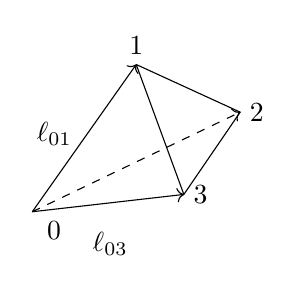
\begin{tikzpicture}[scale=1.1]
\draw[->] (0,0) -- (1.2,1.7);
\draw (1.2,1.7) -- (2.4,1.15) -- (1.75,0.2) -- (1.2,1.7);
\draw[->] (0,0) -- (1.75,0.2);
\draw[dashed,->] (0,0) -- (2.4,1.15);
\node[below] at (0.25,0) {$0$};
\node[above] at (1.2,1.7) {$1$};
\node[right] at (2.4,1.15) {$2$};
\node[right] at (1.75,0.2) {$3$};
\node[left] at (0.57,0.9) {$\ell_{01}$};
\node[below] at (0.9,-0.12) {$\ell_{03}$};
\end{tikzpicture}
\end{adjustbox}
\end{center}
\begin{equation*}
\ell\rightsquigarrow g=(g_{ij}),\qquad
g_{ij}=\frac12(\ell_{0i}^2+\ell_{0j}^2-\ell_{ij}^2)
\end{equation*}
\underline{симметр. и положит. определена}
\begin{equation*}
\mathcal P=\{\text{симм. полож. опр. матрицы }n\times n\}
\end{equation*}
'' $GL(n)/O(n)$
\begin{equation*}
\mathcal M(\sigma^n)=GL(n)/O(n)
\end{equation*}
\underline{Инвар. мера на $\mathcal M(\sigma^n)$}:
\begin{equation*}
\frac{1}{\det g^{\frac{n+1}{2}}}\prod_{i\leq j}dg_{ij} \tag{22}
\end{equation*}
\begin{equation*}
\frac{1}{\operatorname{vol}(\sigma^n,\ell)^{n+1}}\prod d\ell_{ij} \tag{23}
\end{equation*}
— мера на $\mathcal M(\sigma^n)$ (другой способ записи)

\Unclear{GELFAND-P001004}{measure-change}{[В (23) написано $\prod d\ell_{ij}$, без дополнительных множителей.]}
\begin{equation*}
\prod_{x\in M}\operatorname{deg}g(x)^{5/2}\prod_{\mu\leq\nu}dg_{\mu\nu} \tag{24}
\end{equation*}
\Unclear{GELFAND-P001004}{last-measure}{[В (24) буквы похожи на «deg», возможное чтение «det»; показатель $5/2$ — без минуса.]}

\SourcePage{GELFAND-P001005}{unlabelled}
% Review coordinates: original pixels (x0,y0,x1,y1), origin at upper left.
% Enlargements are nearest-neighbour crops, not new source resolution.
% Reviewed top: bbox=(120,30,2250,815); scale=1.5x.
% Reviewed middle: bbox=(125,760,2090,1610); scale=1.5x.
% Reviewed lower: bbox=(130,1555,2020,2200); scale=1.5x.
% Reviewed bottom: bbox=(150,2140,1990,2840); scale=1.5x.
% Reviewed metric-edit: bbox=(890,245,1260,465); scale=4x.
% Reviewed right-cancellation: bbox=(1560,300,2160,440); scale=4x.
% Reviewed induced-verb: bbox=(380,330,920,460); scale=3x.
% Reviewed exponent-comparison: bbox=(520,2145,1560,2320); scale=3x.
% Reviewed chern-name: bbox=(920,850,1210,980); scale=3x.
\begin{equation*}
\mathcal M(P^n)\hookrightarrow\prod_{\sigma^n\subset P^n}\mathcal M(\sigma^n) \tag{25}
\end{equation*}
(подмн-зие)

Возникает индуц. [в строке зачёркнуто:
\Unclear{GELFAND-P001005}{metric-cancel-main}{метрика?};
над строкой вписано, обведено и зачёркнуто:
\Unclear{GELFAND-P001005}{metric-cancel-upper}{кривизна? / метрика?};
ниже обведено: метрика] на $\mathcal M(P^n)$
[зачёркнуто справа: \Unclear{GELFAND-P001005}{right-cancellation}{не удовлетворяющ… [окончание неразборчиво]}]

($\rightsquigarrow$ усл. склеивания)

Вводится мера на пр-ве всех метризаций. $\Rightarrow$ объём, индуцированный рим. метрикой.
\begin{equation*}
P_n\underset{n\to\infty}{\longrightarrow}M
\end{equation*}
(На $\mathcal M(\sigma^n)$ инвар. метрика как на симметрич. пр-ве)

\underline{Идея}: $M^n\subset E^N$ \underline{изометрич.}

Кинематич. ф-ла Чженя:
\begin{equation*}
k=N-n+2,
\end{equation*}
$\mathcal G_{N,k}$ = афф. грассманиан $E^k\subset E^N$

$dE^k$ — мера на $\mathcal G_{N,k}$
\begin{equation*}
\int_{E^k\in\mathcal G_{N,k}}\chi(M^n\cap E^k)dE^k
=c_{N,k}\int_M R\,d\operatorname{vol} \tag{26}
\end{equation*}
\begin{equation*}
\int_{\mathcal G_{N,k}}\chi(P^n\cap E^k)dE^k=c_{N,k}R(P^n) \tag{27}
\end{equation*}
[Под $P^n$ с вертикальной чертой:] симплиц. подмн-зие

[Под правой частью:] (комбинат. скал. кривизна)
\begin{equation*}
P_n\longrightarrow M
\end{equation*}
подинтегр. ф-и в (26) и (27) будут п.в. совпадать.

\begin{center}— . —\end{center}
Для $\displaystyle\int\operatorname{tr}(\Omega^k)$, $k=N-n+2\ell$
\begin{equation*}
\int_{E^k\in\mathcal G_{N,k}}\chi(M^n\cap E^k)dE^k
=c_{N,k}\int_M\operatorname{tr}(\Omega^\ell) \tag{28}
\end{equation*}
\Unclear{GELFAND-P001005}{curvature-exponent}{[В строке перед (28) степень $k$; в правой части (28) — $\ell$.]}
\begin{equation*}
\underset{\text{лев. ч. (27)}}{\text{— '' —}}=c_{N,k}R_\ell(P^n). \tag{29}
\end{equation*}

\SourcePage{GELFAND-P001006}{6}
% Review coordinates: original pixels (x0,y0,x1,y1), origin at upper left.
% Enlargements are nearest-neighbour crops, not new source resolution.
% Reviewed top: bbox=(225,0,2220,510); scale=2x.
% Reviewed lower: bbox=(230,475,2070,1115); scale=2x.
% Reviewed last-line: bbox=(395,940,2040,1050); scale=3x.
% Reviewed local-exact: bbox=(570,485,1870,610); scale=3x.
% Reviewed bottom-marks: bbox=(1670,1040,1980,1230); scale=4x.
\underline{15/II-82}\qquad \underline{Сем. Гельфанда}

\underline{Гинзбург.}

$M$ — симпл. мн-зие

($\omega$ — соотв. 2-форма)

$A$ — группа, действ. на $M$ гамильтоновым образом.

1) $A$ сохраняет $\omega$

$\xi\in\mathfrak A$ — соотв. алгебра Ли

$\xi\longrightarrow\omega(\xi,\cdot)$
\Unclear{GELFAND-P001006}{exactness-word}{локально / глобально}
точна; точна:

2) $\mathfrak A\ni a\longmapsto H_a$\quad (гамильтониан)

гомоморфизм алгебр Ли.

\underline{отобр. момента}: $\mu\colon M\longrightarrow\mathfrak A^*$
\begin{equation*}
m\longmapsto\mu(m),\qquad \mu(m)(a)=H_a(m)
\end{equation*}
[Под аргументом $a$ в $\mu(m)(a)$ написано $\mathfrak A$, стрелка направлена вверх к $a$.]

Перестанов. с действием $A$ и согл. со скобкой Пуассона.

[Под последней строкой справа — две короткие наклонные черты.]

\SourcePage{GELFAND-P001007}{unlabelled}
% Review coordinates: original pixels (x0,y0,x1,y1), origin at upper left.
% Enlargements are nearest-neighbour crops, not new source resolution.
% Reviewed upper: bbox=(120,40,1850,760); scale=2x.
% Reviewed upper-mid: bbox=(220,725,2030,1380); scale=2x.
% Reviewed middle: bbox=(95,1350,2280,2320); scale=2x.
% Reviewed bottom: bbox=(75,2330,2320,3430); scale=2x.
% Reviewed minkowski-note: bbox=(570,430,980,570); scale=4x.
% Reviewed summation-index: bbox=(475,205,790,390); scale=4x.
% Reviewed buffon-cancellation: bbox=(510,1375,690,1450); scale=6x.
% Reviewed para-caption: bbox=(1160,1740,1430,1885); scale=4x.
% Reviewed volume-word: bbox=(1420,1895,1710,2000); scale=4x.
% Reviewed macmullen: bbox=(255,2210,1240,2340); scale=3x.
% Reviewed integral-link: bbox=(520,910,1160,1035); scale=3x.
% Reviewed para-diagram: bbox=(30,1760,480,2120); scale=3x.
% Reviewed young-diagram: bbox=(895,2705,1640,3150); scale=3x.
% Reviewed volume-abbreviation: bbox=(1160,1895,1450,2010); scale=4x.
\underline{22/II-82г.}\qquad \underline{Сем. Гельфанда}

\underline{Арнольд.}

\begin{equation*}
V(\varepsilon)=\sum_{i=0}^{n}V_k\varepsilon^k,
\qquad
\sigma_i(k)=\sum_{C_n^i}k_1\ldots k_i
\end{equation*}
\Unclear{GELFAND-P001007}{summation-index}{Внизу суммы $i=0$; в слагаемом $V_k\varepsilon^k$.}

[Под $V(\varepsilon)$:] объём ($\varepsilon$-оболочка вып. тела)

(Теорема Минковского — это многочлен)

$k_s$ — соб. числа $\dfrac{2\ \text{кв. ф.}}{1\ \text{кв. ф.}}$

\begin{equation*}
V_i=C_i\int_{\partial D}\sigma_i(k)\,dS
\end{equation*}

\begin{equation*}
V_k=\widetilde C_k\int_{\xi\in G_{n,k}}\operatorname{mes}(\pi_\xi D)\,d\xi,
\qquad \pi_\xi\colon R^n\longrightarrow\xi
\end{equation*}
[Под интегралом проведена горизонтальная скобка с загнутыми вверх концами;
под ней две короткие наклонные черты. Ниже:]
\begin{equation*}
\int_{H_{n,k}}\chi(h\cap D)\,dh
\end{equation*}

$H_{n,k}$ — все плоск., не обязательно прох. через $0$

$\chi$ — эйлерова хар-ка.

\underline{Это способ}
[зачёркнуто: \Unclear{GELFAND-P001007}{buffon-cancellation}{Бюф\ldots}]
\underline{Бюффона} (и потом обобщил Сантало)

[Под словами «способ Бюффона»:] вычисления числа $\pi$

Вычисление констант $C_k$, $\widetilde C_k$ — с помощью шаров.

\underline{Переносится на решётчатый случай.}

Вместо объёма — число целых точек.

\underline{целочисл. параллелограм}
(\Unclear{GELFAND-P001007}{parallelogram-caption}{-липед / мног\ldots})

\SourceFigure{GELFAND-P001007}{parallelogram-diagram}{На левом поле наклонный параллелограмм с отмеченными четырьмя вершинами. Нижняя наклонная сторона продолжена пунктиром в обе стороны. У правой нижней вершины небольшой петлеобразный штрих: часть отметки вершины или отдельный знак $0$; требуется сверка этого штриха с оригиналом. Подписей у остальных вершин не видно.}

Объём параллелепипеда — число, показ., сколько элемент. пар.-липедов.

На прямой возникает решётка из пересечений

Надо взять факторпр-во и это даёт аналог высоты.

(там тоже есть аналог решётки)

\underline{Mac Mullen} доклад в
[зачёркнуто: \Unclear{GELFAND-P001007}{vancouver-cancellation}{Ванку\ldots}]
Ванкувере — там есть лит-ра.

\underline{И. М. Гельфанд.}

\underline{О книге Mc Donald'а} «Симметрические ф-и и полиномы Холла»

\underline{Задача.} Рассм. разбиение (partition)
\begin{equation*}
(L)\qquad \lambda_1\geq\lambda_2\geq\ldots\geq\lambda_k
\qquad (\text{целые числа})
\end{equation*}

Разреш. дописывать нули.

Способы записи: $(L)$ или
\begin{equation*}
\begin{array}{rccccc}
5&\bullet&\bullet&\bullet&\bullet&\bullet\\
4&\bullet&\bullet&\bullet&\bullet&\\
4&\bullet&\bullet&\bullet&\bullet&\\
1&\bullet&&&&
\end{array}
\end{equation*}

% Source geometry: x=895..1640, y=2705..3150; inspected at 3x.
\begin{center}
\begin{adjustbox}{max width=\linewidth}
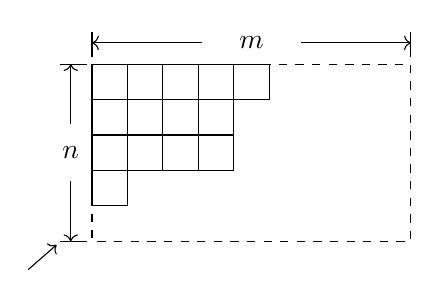
\begin{tikzpicture}[x=0.45cm,y=0.45cm]
\draw[dashed] (0,0) rectangle (9,-5);
\draw (0,0)--(5,0)--(5,-1)--(4,-1)--(4,-3)--(1,-3)--(1,-4)--(0,-4)--(0,0);
\draw (0,-1)--(4,-1);
\draw (0,-2)--(4,-2);
\draw (0,-3)--(1,-3);
\draw (1,0)--(1,-3);
\draw (2,0)--(2,-3);
\draw (3,0)--(3,-3);
\draw (4,0)--(4,-1);
\draw (0,0.2)--(0,0.9);
\draw (9,0.2)--(9,0.9);
\draw[->] (3.1,0.6)--(0,0.6);
\draw[->] (5.9,0.6)--(9,0.6);
\node at (4.5,0.6) {$m$};
\draw (-0.9,0)--(-0.15,0);
\draw (-0.9,-5)--(-0.15,-5);
\draw[->] (-0.6,-1.7)--(-0.6,0);
\draw[->] (-0.6,-3.3)--(-0.6,-5);
\node at (-0.6,-2.5) {$n$};
\draw[->] (-1.8,-5.8)--(-1,-5.1);
\end{tikzpicture}
\end{adjustbox}
\end{center}

Вместо точек — квадратики лучше (схемы Юнга)

Поместим в пр-к размерами $m\times n$ и рассм. числа

\SourcePage{GELFAND-P001008}{11}
% Review coordinates: original pixels (x0,y0,x1,y1), origin at upper left.
% Enlargements are nearest-neighbour crops, not new source resolution.
% Reviewed upper: bbox=(85,15,2190,835); scale=2x.
% Reviewed upper-mid: bbox=(65,795,2250,1640); scale=2x.
% Reviewed middle: bbox=(125,1595,2290,2470); scale=2x.
% Reviewed lower: bbox=(40,2450,2240,3410); scale=2x.
% Reviewed generating-function: bbox=(920,700,1240,850); scale=4x.
% Reviewed author-name: bbox=(230,875,520,985); scale=5x.
% Reviewed local-word: bbox=(250,1340,565,1450); scale=4x.
% Reviewed quantize-contact: bbox=(305,1500,2235,1610); scale=3x.
% Reviewed theorem-lines: bbox=(190,1610,2205,1810); scale=3x.
% Reviewed quantization-cancel: bbox=(700,1770,1175,1865); scale=5x.
% Reviewed w-definition: bbox=(270,2750,1150,2845); scale=3x.
% Reviewed w-subscript: bbox=(1345,2765,1490,2880); scale=6x.
% Reviewed w-small: bbox=(1450,2760,1595,2895); scale=6x.
% Reviewed contact-word: bbox=(1140,1505,1460,1605); scale=5x.
% Reviewed quantize-word: bbox=(315,1510,630,1610); scale=4x.
% Reviewed quant-symbols: bbox=(970,1870,1435,1965); scale=4x.
% Reviewed integral-function: bbox=(1335,2320,1530,2450); scale=4x.
\begin{equation*}
(*)\quad\left\{
\begin{array}{ll}
\lambda_i+n-i,&1\leq i\leq n,\\
n-1+j-\lambda'_j,&1\leq j\leq m
\end{array}\right.
\end{equation*}

$\lambda'=4,3,3,3,1$ — двойств. картинка

\underline{Задача:}

Набор из $m+n$ чисел $(*)$ — перестановка чисел $0,1,2,\ldots,m+n-1$.

\underline{Следствие.}
\begin{equation*}
f_{\lambda,n}(t)\overset{\mathrm{def}}{=}\sum_{i=1}^{n}t^{\lambda_i+n-i}
\end{equation*}
Тогда
\begin{equation*}
f_{\lambda,n}(t)+t^{m+n-1}f_{\lambda,m}(t)=\frac{1-t^{m+n}}{1-t}
\end{equation*}
\Unclear{GELFAND-P001008}{generating-function}{Во втором слагаемом написано $f_{\lambda,m}(t)$, без видимого штриха у $\lambda$ и без отрицательной степени аргумента.}

\underline{И. М. Гельфанд} с раб.

\Unclear{GELFAND-P001008}{author-name}{Гийемина / Гийлемина}

\underline{Новые усл-ия асимпт. ф-лы Вейля}

\underline{Симпл. конус:}\qquad $\rho_a^*\omega=a\omega$,\quad $a>0$.

\underline{Пример 1.} $R^{2n}=\{(x,\xi)\}$,
$x\in R^n$, $\xi\in(R^n)^*$,
$\rho_a(x,\xi)=(a^{1/2}x,a^{1/2}\xi)$

\underline{Пример 2.} $T^*X$\qquad $a(x,\xi)=(x,a\xi)$

\underline{Арнольд.}

Локально все конусы одинаковы: фактор — контактное мн-зие.

(Симпл. конусы $\Longleftrightarrow$ конт. мн-зия)

Квантование надо именно
\Unclear{GELFAND-P001008}{contact-ending}{контактное / контактные},
т.к. надо действие — \underline{1-форму!!}

\underline{Утв.} Всегда квантуется и единственным обр.
\Unclear{GELFAND-P001008}{construction-abbreviation}{стр. / опр.}
алг. Вейля,
микролокально существ. и топол. (микролокально) классич. алг. Вейля.

\underline{Квантование} —
[зачёркнуто: \Unclear{GELFAND-P001008}{quantization-cancellation}{набор\ldots\ [остальное неразборчиво]}]

\begin{equation*}
x_k\longmapsto x_k,\qquad \xi_k\longmapsto i\frac{\partial}{\partial x_k}.
\end{equation*}
\begin{equation*}
p(x,\xi)=\sum_{i=0}^{\infty}p_i(x,\xi),
\qquad p_i\text{ — однор. степ. }2\mu-2i
\end{equation*}
\begin{equation*}
\rho_a(x,\xi)=(a^{1/2}x,a^{1/2}\xi);\qquad \mu\in C.
\end{equation*}
(Это символ порядка $\mu$).
\begin{equation*}
(Pf)(x)=(2\pi)^{-n}\int p\left(\frac{x+y}{2},\xi\right)e^{i\xi\cdot(x-y)}u(y)\,dy\,d\xi
\end{equation*}
\Unclear{GELFAND-P001008}{quantization-convention}{Слева $(Pf)(x)$, в интеграле $u(y)$; выше образ $\xi_k$ записан с положительным $i$.}

$W^\mu$ — пр-во таких операторов,\qquad $\underline{W^{\mu-1}\subset W^\mu}$.

\underline{Символ:} элемент $W^\mu/W^{\mu-1}$

$H$ — гильб. пр-во, $S$ — плотное подпр-во, где действ. все такие опер.

$\underline W^\mu$ — соотв. пр-во оп.
(вида $A_1+\cdots+A_k$, $A_i\in W^{\mu_i}$
\Unclear{GELFAND-P001008}{w-subscript}{Под $W$ маленький перечёркнутый или надписанный индекс: $\mathrm{cl}$ / $00$ / неразборчиво.}
в примере)

\underline{Аксиомы:}

[Слева вертикальная скобка с подписью «группа $A$».]
\begin{align*}
1)\quad &\underline W^\mu\supset\underline W^{\mu-1}\\
2)\quad &A\in\underline W^\mu,\quad B\in\underline W^\nu
\ \Longrightarrow\ AB\in\underline W^{\mu+\nu}\\
3)\quad &A\in\underline W^\mu,\quad B\in\underline W^\nu
\ \Longrightarrow\ [A,B]\in\underline W^{\mu+\nu-1}\\
4)\quad &A\in\underline W^\mu\ \Longrightarrow\ A^*\in\underline W^{\bar\mu}\\
5)\quad &I\in\underline W^0
\end{align*}

\SourcePage{GELFAND-P001009}{unlabelled}
% Review coordinates: original pixels (x0,y0,x1,y1), origin at upper left.
% Enlargements are nearest-neighbour crops, not new source resolution.
% Reviewed upper: bbox=(180,20,1895,715); scale=2x.
% Reviewed lower: bbox=(290,720,2310,1470); scale=2x.
% Reviewed exact-note: bbox=(350,1065,1325,1185); scale=3x.
% Reviewed product-argument: bbox=(855,1325,1135,1430); scale=5x.
[Слева квадратная скобка у пункта 6).]
\begin{gather*}
6)\quad\forall A_i\in\underline W^{\mu-i},\quad i=0,1,2,\ldots\\
\Longrightarrow\ \exists A\in\underline W^\mu,\qquad
A-\sum_{i=0}^{N-1}A_i\in\underline W^{\mu-N}.
\end{gather*}

\underline{Группа $B$.}

$1^{\circ}$. Если $\operatorname{Re}\mu\leq0$, то $\forall A\in\underline W^\mu$ ограничен.

$2^{\circ}$. Если $\operatorname{Re}\mu<0$, то $\forall A\in\underline W^\mu$ компактен.

$3^{\circ}$. $\exists s_0>0$, если $A\in\underline W^\mu$,
$\operatorname{Re}\mu<-s_0$, то $A$ ядерный

\underline{Группа $C$.}
\begin{equation*}
A\in\underline W^0,\quad A\text{ компактен}
\ \Longrightarrow\ A\in\underline W^{-1}
\end{equation*}

\underline{$D$.} Точная посл.

% Source geometry: x=370..1560, y=975..1090; inspected within a 2x band.
\begin{center}
\begin{adjustbox}{max width=\linewidth}
\begin{tikzcd}
0\arrow[r]&\underline W^{\mu-1}\arrow[r]&\underline W^\mu\arrow[r]&
\underline W^\mu/\underline W^{\mu-1}\arrow[r]&0
\end{tikzcd}
\end{adjustbox}
\end{center}

«хорошо» разлож. в прямую сумму.

\underline{$E$.}\qquad $\exists A(\mu)\in\underline W^\mu$, аналит. завис. от $\mu\in C$,
такой что $A(0)-I\in\underline W^{-1}$ и
\begin{equation*}
A(\mu)A(\nu)-A(\nu+\mu)\in\underline W^{\mu+\nu-1}.
\end{equation*}

\SourcePage{GELFAND-P001010}{15}
% Review coordinates: original pixels (x0,y0,x1,y1), origin at upper left.
% Enlargements are nearest-neighbour crops, not new source resolution.
% Reviewed upper: bbox=(60,20,2270,670); scale=2x.
% Reviewed upper-mid: bbox=(175,620,2210,1250); scale=2x.
% Reviewed middle: bbox=(100,1200,2250,2410); scale=2x.
% Reviewed lower: bbox=(50,2370,2320,3440); scale=2x.
% Reviewed title-cancel: bbox=(990,165,1175,240); scale=5x.
% Reviewed sheaves-word: bbox=(475,245,725,345); scale=5x.
% Reviewed holonomic-word: bbox=(990,240,1350,355); scale=5x.
% Reviewed parenthetic: bbox=(195,320,520,475); scale=4x.
% Reviewed closed-ending: bbox=(900,2825,1170,2940); scale=5x.
% Reviewed diagram-lower: bbox=(35,2930,800,3215); scale=4x.
% Reviewed lower-cancellation: bbox=(1370,3025,1555,3105); scale=6x.
% Reviewed bottom-line: bbox=(105,3310,1890,3420); scale=3x.
\underline{1/III-82.}\qquad \underline{Сем. Гельфанда.}

\underline{R. MacPherson.}\quad \underline{The title of a paper}
[зачёркнуто: \Unclear{GELFAND-P001010}{title-cancellation}{which / what}]
\underline{he would speak about:}

\begin{equation*}
\text{Perverse Sheaves}\ \approx\ \text{Holonomes }D\text{-modules}
\end{equation*}
[Под «Perverse»:] (извращенные ?)

[Ниже слева:] (катег.

\SourceFigure{GELFAND-P001010}{title-diagram}{Вверху подчёркнуты «Perverse Sheaves» и «Holonomes $D$-modules», между ними знак $\approx$. Под ними справа подпись «char variety». От правого заглавия к ней вниз идёт волнистая стрелка; от левого заглавия вниз вправо идёт пунктирная стрелка, под ней знак вопроса. Окончание слова в правом заглавии читается «Holonomes», но требует проверки против «Holonomic»; преждевременная нормализация подписи не сделана.}

\underline{Другой заголовок:}

$H(X\longrightarrow Y)$\qquad \underline{теория гомол. отображений пр-в.}
\begin{align*}
H(X\longrightarrow pt)&=H_*(X)\\
H(X\overset{\mathrm{id}}{\longrightarrow}X)&=H^*(X)
\end{align*}

% Source geometry: x=300..730, y=1030..1200; inspected in a 2x band.
\begin{center}
\begin{adjustbox}{max width=\linewidth}
\begin{tikzcd}
X\arrow[r]\arrow[rr,bend right=25]&Y\arrow[r]&Z
\end{tikzcd}
\end{adjustbox}
\end{center}
\underline{есть умножение}, накрыв. композ. отобр.

\underline{D. McDuff.}\qquad \underline{Когом. группы диффеом., сохр. объём.}

\begin{equation*}
\mathcal G=\operatorname{Diff}_{\omega 0}^{c}M,
\end{equation*}
$\omega$ — форма объёма на $M$, $M$ — мн-зие;

$c$ — с комп. носителем; $0$ — связная компонента $Id$.

$\mathcal G$ с обычной топологией $(C^\infty)$.

$G$ — та же гр. в дискр. топ.
\begin{equation*}
G\underset{\text{тожд.}}{\longrightarrow}\mathcal G
\end{equation*}

[Над $BG$ следующей строки написано $K(G,1)$, под этой подписью две короткие вертикальные черты.]
\begin{equation*}
\overline B\mathcal G\longrightarrow BG\longrightarrow B\mathcal G
\qquad (\text{классиф. пр-ва})
\end{equation*}
[От $\overline B\mathcal G$ короткий вертикальный штрих к подписи:]

гомот. слой (превр. отобр. в расслоение, тогда $\overline B\mathcal G$ — слой)

$\overline B\mathcal G$ зав. только от окр. $1$ в $\mathcal G$

Это топологич. версия алг. Ли в нек-ром смысле

\underline{Фукс:}
\begin{equation*}
G/H\longrightarrow BH\longrightarrow BG
\end{equation*}
(обычно); если $H$ [вставлено над строкой: очень] плотно в $G$,
то фунд. область — «инфинитезим.» окр. единицы

$\overline B\mathcal G\times M$ имеет слоение $\mathcal F$,
трансверс. ко всем слоям $x\times M$
и определяемое [вставлено: такой] замкнутой
\Unclear{GELFAND-P001010}{closed-form-overwriting}{Окончание «замкнутой» написано по другим штрихам; прежнее окончание неразборчиво.}
$n$-формой $\Omega$, что $\Omega|_{x\times M}=\omega$.

\SourceFigure{GELFAND-P001010}{bundle-diagram}{Внизу слева три вертикальные стрелки вниз. Верхние подписи слева направо: $E'\simeq\overline B\mathcal G\times M$, $E'$, $E$; в левой подписи знак между $\mathcal G$ и $M$ тесно слит с буквами. Нижние подписи соединены стрелками вправо: $\overline B G\longrightarrow BG\longrightarrow B\mathcal G$. У средней и правой вертикальных стрелок написано $M$; над правой подписью $M$ имеется густо зачёркнутая запись, также похожая на $M$. В левой нижней подписи $G$ выглядит обычным прописным, в отличие от рукописного $\mathcal G$ в верхней подписи. Сверить штрихи, штрихи у $E'$ и различие $G/\mathcal G$; не добавлять отсутствующие горизонтальные стрелки в верхнем ряду.}

$E$ — станд. расслоение со слоем $M$

$E'$ — его подъём,
[зачёркнуто: \Unclear{GELFAND-P001010}{connection-cancellation}{связность / с\ldots}]
у него $0$-я кривизна,
т.к. слой соотв. главного рассл. дискретен.

Слева — огранич. на слой — оно стан. трив. по св-ву классиф. пр-ва.

Связн. $0$-й кривизны переносится и даёт слоение на $\overline B\mathcal G\times M$


% Дипломатическая транскрипция; координаты (x0,y0,x1,y1) отсчитываются от
% левого верхнего угла исходного PNG 2408 x 3496; увеличение растровое.
\SourcePage{GELFAND-P001011}{unlabelled}
% Просмотрен весь оригинал, включая поля и нижнюю незаписанную часть.
% Общие просмотры: (240,25,1830,770) x3; (330,700,2240,1380) x3;
% (360,1320,2050,2120) x3; (320,2110,2200,3360) x3.
% Повторно: (880,200,1180,365) x8; нижний индекс первой omega прочитан 0.
$\Omega-\pi^*\omega=0$ вблизи $\infty$ на $M$.

Классы.
\begin{equation*}
c_k(M)\in H^k\left(\bar B\operatorname{Diff}^{c}_{\omega_0}M;
\underset{\substack{\vert\\\text{коэффициенты}}}{H_c^{n-k}(M;\mathbb R)}\right)
\end{equation*}
$n=\dim M$.

Пусть $K$ — $k$-цикл в $\bar B\operatorname{Diff}^{k}_{\omega_0}M$
\Unclear{GELFAND-P001011}{upper-diff-superscript}{[Видимый верхний индекс $k$ сохранён; его отличие от $c$ в соседних формулах не устранено.]}
\begin{equation*}
c_k(M)(K)=\text{класс замкнутой }(n-k)\text{-формы }
 x\longmapsto\int_{K\times x}\Omega
\end{equation*}

\underline{Пример.} $M=T^n$, $K=T^n$.
\begin{equation*}
\begin{aligned}
T^n\times T^n&\longrightarrow T^n\\
(x,y)&\longmapsto x+y
\end{aligned}
\end{equation*}
Берем [зачёркнуто: слоение на $T^n$ и
\Unclear{GELFAND-P001011}{middle-cancelled-verb}{поднимем / поднимаем (неуверенно)}]
[вставлено сверху в обведённой выноске: возник. слоение]
на $T^n\times T^n$. Получ. слоение,
предст. цикл. в $\bar B\operatorname{Diff}^{c}_{\omega_0}T^n$.
\begin{equation*}
c_n(T^n)(T^n)=\int_{T^n\times x}\Omega
\qquad\text{не зав. от выбора }x.
\end{equation*}

\underline{Предл.} 1
\begin{equation*}
\begin{aligned}
c_n(S^n)&=0\quad\text{при чётном }n\\
&\ne0\quad\text{при нечётном }n
\end{aligned}
\end{equation*}
\underline{1-е утв.:}
$K^n\times S^n$\qquad ($K^n$ — любое мн-зие)

% Рисунок: шесть почти вертикальных отрезков; нижний поперечный отрезок
% и верхняя плавная кривая. Источник: (620,1690,850,1810), просмотр x3.
\begin{adjustbox}{max width=\linewidth}
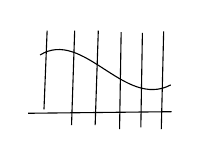
\begin{tikzpicture}[x=1cm,y=1cm]
\draw (0,0.05)--(0.04,1.05);
\draw (0.35,-0.15)--(0.39,1.05);
\draw (0.65,-0.15)--(0.69,1.05);
\draw (0.96,-0.2)--(0.98,1.03);
\draw (1.23,-0.18)--(1.25,1.02);
\draw (1.49,-0.2)--(1.52,1.04);
\draw (-0.2,0)--(1.62,0.02);
\draw (-0.05,0.74)..controls (0.5,1.08) and (1.02,0.05)..(1.61,0.36);
\end{tikzpicture}
\end{adjustbox}
\quad $\Omega$ — форма, зад. слоение, трансверс. сферам
\begin{equation*}
\text{Тогда }\int_{\substack{\text{гориз.}\\\text{слой}}}\Omega=0.
\end{equation*}
Стр. другой класс $s$

\underline{Предл.} 2
\begin{equation*}
\begin{aligned}
s(\mathbb R^n)&\ne0\quad n\text{ чётно}\\
&=0\quad n\text{ нечётно}
\end{aligned}
\end{equation*}

\underline{\underline{Milnor}}.

$G$ — гр. Ли, $G^\delta$ — та же с дискр. топологией
\begin{equation*}
\begin{gathered}
G^\delta\longrightarrow G\\
BG^\delta\longrightarrow BG
\end{gathered}
\end{equation*}
\begin{equation*}
H_*\left(\qquad\begin{matrix}\mathbb Q\\\mathbb Z\\\mathbb Z_p\end{matrix}\right)\ -\ ?
\end{equation*}
% В предыдущей записи после открывающей скобки действительно пустое место;
% Q, Z, Z_p записаны столбцом у правой скобки; аргумент не дополнялся.
$H_*(BG)$ хорошо изв. и хорошо себя ведут

$H_*(BG^\delta)$ — ?

неизвестны и нехорошо себя ведут;
неясно, полезны ли?

В алгебр. $K$-теории, в теории слоений, в 3-й пробл. Гильберта
— всё это возникает.\qquad (равносоставленность)

\SourcePage{GELFAND-P001012}{16}
% Полный оригинал просмотрен, верхний правый номер непосредственно прочитан 16.
% Общие просмотры: (150,0,2300,835) x3; (250,805,1540,1460) x3;
% (180,1440,2290,2740) x3; (200,2660,2408,3496) x3.
\underline{Гипотеза об изоморфизме:}
\begin{equation*}
(1)\qquad
H_*(BG^\delta,\mathbb Z/p)\overset{\simeq}{\longrightarrow}H_*(BG,\mathbb Z/p);
\qquad \underline{\forall\ \text{простого }p.}
\end{equation*}
К 3-й пробл. Гильб. это применили H. Sah, Dupont

Когда равносоставимы? Частичн. ответ — из когомологий классиф. пр-ва

Вероятно (1) — очень трудное утв.

\underline{Chern-Weyl:} $G$ компактна $\Rightarrow$
\begin{equation*}
\widetilde H_*(BG^\delta,\mathbb Q)\overset{0}{\longrightarrow}\widetilde H_*(BG,\mathbb Q).
\end{equation*}
(отобр. тривиально)

\underline{Sah-}\Unclear{GELFAND-P001012}{upper-sah-name}{\underline{Wagener / Wagoner (неуверенно)}}:
\begin{equation*}
\underset{\text{связна}}{G}\ne1\quad\Rightarrow\quad\exists\ \text{эпиморфизм}
\end{equation*}
\begin{equation*}
H_2(BG^\delta,\mathbb Z)\longrightarrow
\underset{\substack{\text{несчёт.}\\\text{сумма}}}{\coprod}\mathbb Q\longrightarrow0
\end{equation*}
В то же время:

$H_2(BG,\mathbb Z)$ конечно порождена.

\underline{Обсудим свид. в пользу (1).}

\tikz{\node[draw,circle,inner sep=1pt]{1};}
(1) верно в спец. случае, если алг. Ли $\mathfrak g$ разрешима

Д-во элементарно
\begin{equation*}
\begin{gathered}
\bar B G\longrightarrow BG^\delta\longrightarrow BG
\end{gathered}
\end{equation*}
[Под $\bar B G$ проведена короткая вертикальная черта к записи:]
по инд. док., что когом. $\bar B G$ трив.,

\tikz{\node[draw,circle,inner sep=1pt]{2};}
Пусть $G$ им. конечное число компонент.

Тогда (1) — эпим. и расщепляется
\begin{equation*}
H_*(BG^\delta,\mathbb Z/p)
\underset{\underline{\mathrm{split}}}{\longrightarrow}
H_*(BG,\mathbb Z/p)\longrightarrow0
\end{equation*}
\Unclear{GELFAND-P001012}{middle-arrow-cancellation}{[Над первой стрелкой зачёркнуто: эп. (неуверенно); остальное неразборчиво.]}

\Unclear{GELFAND-P001012}{left-margin-cancelled-number}{[Слева от (2) отдельный петлеобразный, перечёркнутый знак; неразборчиво.]}
(2)\quad \underline{Следствие.}
\begin{center}
\begin{adjustbox}{max width=\linewidth}
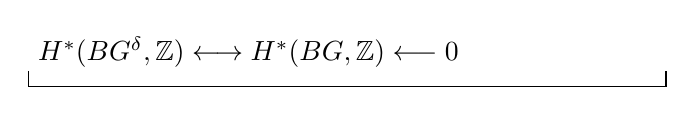
\begin{tikzpicture}
\node[anchor=south west] at (0,0.12) {$H^*(BG^\delta,\mathbb Z)\longleftrightarrow H^*(BG,\mathbb Z)\longleftarrow0$};
\draw (0,0.2)--(0,0)--(8.1,0)--(8.1,0.2);
\end{tikzpicture}
\end{adjustbox}
\end{center}
\Unclear{GELFAND-P001012}{middle-cohomology-arrow}{[У стрелки между двумя группами видны оба наконечника; это начертание сохранено, направление отображения не исправлялось.]}

Общ. — теор.
[зачёркнуто: \Unclear{GELFAND-P001012}{lower-bott-cancellation}{Ду / неразборчиво}]
Bott-Heitsch

% Отменённое «при» проверено в (875,2665,1025,2775), увеличение 10×.
\tikz{\node[draw,circle,inner sep=1pt]{3};}
(1) всегда верно [зачёркнуто: при] для $H_1$ и в интересных случаях для $H_2$:
\begin{equation*}
\operatorname{SL}_n\mathbb R,\quad \operatorname{SL}_n\mathbb C.
\end{equation*}
\Unclear{GELFAND-P001012}{lower-sl-cancellation}{[Между индексом $n$ и $\mathbb R$ зачёркнут опущенный вниз символ: $\mathbb Z$ (неуверенно).]}

\underline{Хефлигер.}

$\operatorname{PSL}_2(\mathbb Z)$ на $\operatorname{Im}z>0$.

(др.-лин. преобр. [зачёркнуто: \Unclear{GELFAND-P001012}{lower-fractional-cancellation}{ко / неразборчиво}] с целыми коэфф.)

% Круг и все подписи просмотрены в (1780,2910,2300,3200) x4.
\begin{adjustbox}{max width=\linewidth}
\begin{tikzpicture}[x=1cm,y=1cm]
\draw (0,0) circle[radius=0.55];
\node[anchor=west] at (0.85,0.15) {прямая —};
\node[anchor=west] at (0.85,-0.2) {— окр.};
\node[anchor=west] at (-0.2,-0.85) {$S^1$ — гран.};
\end{tikzpicture}
\end{adjustbox}

$\gamma_1,\gamma_2$ — \underline{образующие}.
\begin{equation*}
\gamma_1:z\longmapsto z+1;\qquad
\gamma_2:z\longmapsto-\frac{1}{z}.
\end{equation*}
% Знак вопроса при exists проверен в (550,3160,920,3340) x6:
% это высокий ?, с отдельной точкой снизу; сохранён как вопрос автора.
$\forall f\in C^\infty(S^1),\quad\exists?\ C^\infty$-ф-и $f_1,f_2\in C^\infty(S^1)$

\SourcePage{GELFAND-P001013}{unlabelled}
% Просмотрен весь оригинал 2408 x 3496; запись занимает только верхние
% приблизительно 500 пикселей; рукописной метки страницы нет.
% Общий просмотр (130,25,2300,520) x3; повторные просмотры:
% (1160,175,1610,275) x6 -> рим.; (1990,175,2290,270) x6 -> мин;
% (950,360,1480,485) x6 -> аппроксимировать.
\begin{equation*}
(1)\qquad f(x)=f_1(x)-f_1(\gamma_1(x))+f_2(x)-f_2(\gamma_2(x)).
\end{equation*}
Это связано со слоениями на рим. мн-зии, слои к-рых явл. \underline{мин} пов.

\underline{Неизвестно}!

Приблизительно верно: аппроксимировать можно (в $C^\infty$-топ.) — это легко.

\SourcePage{GELFAND-P001014}{unlabelled}
% Original inspected at 2408 x 3496, including blank upper region. Enlarged text: (120,2390,2270,2880) 3x; (130,2860,2290,3370) 3x; name (1320,2580,2408,2730) 5x; example (210,2880,1090,3010) 5x; bibliography (360,2760,1130,2870) 4x. Coordinates are original pixels, left/top/right/bottom.
15/\underline{III}-82. \underline{Сем. Гельфанда.}

\underline{Темы} (курсовых работ, дипл. работ и т. д.)

\underline{Кириллов}:

\begin{adjustbox}{max width=\linewidth}
\begin{tikzpicture}
\node[anchor=east] at (0,0) {1. \underline{Кратность веса}};
\draw (0.1,0.12) -- (0.7,0.45);
\draw (0.1,-0.1) -- (0.7,-0.1);
\node[anchor=west,align=left] at (0.9,0.5) {комп. группы Ли $\to$ Гийемин, Стернберг\quad в принципе\\получили ответ.};
\node[anchor=west] at (0.9,-0.3) {гиперболич. алгебры};
\end{tikzpicture}
\end{adjustbox}

\underline{Лит-ра}: \underline{Мак-дональд} (статья)

\underline{Пример} \underline{зад.} в \underline{2}: рассм. контрагредиентная алгебра Ли с гиперболич.
матрицей Картана (имеющей отриц. соб. значение)

Рассм. действие $SU(3)$ на её алгебре Ли:
\begin{equation*}
X=\begin{pmatrix}
i\varphi_1&a&c\\
-\bar a&i\varphi_2&b\\
-\bar c&-\bar b&i\varphi_3
\end{pmatrix},\qquad
\varphi_1+\varphi_2+\varphi_3=0
\end{equation*}
\begin{equation*}
g\in SU(3)\Rightarrow g:X\to gXg^*.
\end{equation*}

\SourcePage{GELFAND-P001015}{unlabelled}
% Original inspected at 2408 x 3496. Full-page text reviewed in enlarged 3x strips (150,15,2350,640), (160,610,2320,1440), (140,1420,2320,2160), (190,2110,2320,3030), (160,3020,2350,3470). Further symbol/diagram coordinates and scales are recorded in the ledger.
Рассм. орбиту $\Omega$.
\Unclear{GELFAND-P001015}{orbit-punctuation}{[отдельный штрих: 1 / !]}
Она имеет вид:
\begin{equation*}
\begin{cases}
\operatorname{tr}\ \Unclear{GELFAND-P001015}{trace-cancellation}{[зачёркнутый знак неразборчив]}\ X^2=c_2,\\
\operatorname{tr}X^3=c_3
\end{cases}
\qquad (\text{и, кстати, }\operatorname{tr}X=0)
\end{equation*}
(по этим следам восстан. корни,
а $\forall$ матр. привод. к диаг. виду)

Обозначим её: $\Omega_{c_2,c_3}$.

Орбита — размерности 6 (общ. полож.)

Спроектир. на плоскость (2-мерн.) $(\varphi_1,\varphi_2,\varphi_3)$,
$\varphi_1+\varphi_2+\varphi_3=0$.

% Three-ray drawing: original (430,590,890,955), examined in full image and 3x upper/middle crops.
\begin{adjustbox}{max width=\linewidth}
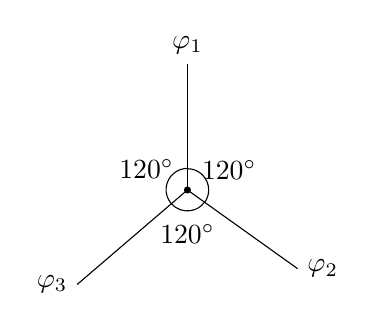
\begin{tikzpicture}
\draw (0,0) -- (0,1.6) node[above] {$\varphi_1$};
\draw (0,0) -- (1.4,-1.0) node[right] {$\varphi_2$};
\draw (0,0) -- (-1.4,-1.2) node[left] {$\varphi_3$};
\fill (0,0) circle (0.045);
\draw (0,0.27) arc[start angle=90,end angle=-36,radius=0.27];
\draw (-0.208,-0.17) arc[start angle=220,end angle=90,radius=0.27];
\draw (-0.208,-0.17) arc[start angle=220,end angle=324,radius=0.27];
\node at (-0.52,0.27) {$120^{\circ}$};
\node at (0.53,0.25) {$120^{\circ}$};
\node at (0,-0.56) {$120^{\circ}$};
\end{tikzpicture}
\end{adjustbox}

\SourceFigure{GELFAND-P001015}{cancelled-axes}{[Зачёркнутый набросок под рисунком трёх осей: вверх направлена стрелка; справа внизу видны петлеобразные следы подписи и несколько пересекающихся штрихов. Исходная геометрия и подписи под зачёркиванием не читаются уверенно.]}

— проектируем на плоскость $\varphi_1+\varphi_2+\varphi_3=0$
\Unclear{GELFAND-P001015}{projection-cancellation}{[зачёркнуто: неразборчиво]}
оси координат.

— так надо рисовать.\qquad ($p$ — проекция)

\underline{Факты}:

а) Проекция $\Omega_{c_1,c_2}$ заполняет 6-угольник.
\Unclear{GELFAND-P001015}{orbit-indices}{[В этой строке написано $c_1,c_2$; выше орбита обозначена индексами $c_2,c_3$.]}

% Hexagon and axes: original (300,1170,760,1570), examined at 4x. Three dashed interior segments and three outgoing coordinate arrows are preserved.
\begin{adjustbox}{max width=\linewidth}
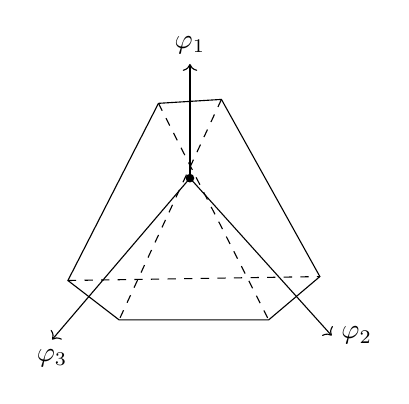
\begin{tikzpicture}
\draw (-0.4,1.3) -- (0.4,1.35) -- (1.65,-0.9) -- (1.0,-1.45) -- (-0.9,-1.45) -- (-1.55,-0.95) -- cycle;
\draw[dashed] (-0.4,1.3) -- (1.0,-1.45);
\draw[dashed] (0.4,1.35) -- (-0.9,-1.45);
\draw[dashed] (-1.55,-0.95) -- (1.65,-0.9);
\draw[->] (0,0.35) -- (0,1.8) node[above] {$\varphi_1$};
\draw[->] (0,0.35) -- (1.8,-1.65) node[right] {$\varphi_2$};
\draw[->] (0,0.35) -- (-1.75,-1.7) node[below] {$\varphi_3$};
\fill (0,0.35) circle (0.055);
\end{tikzpicture}
\end{adjustbox}

(это мн-во диаг. элементов матриц с фиксир.
набором соб. значений $\lambda_1,\lambda_2,\lambda_3$)

б) \underline{Рассм.} $p^{-1}(y_0)$, $y_0$ — точка 6-угольника.

Это \Unclear{GELFAND-P001015}{fibre-dimension}{4-мерное / 4+ мерное} мн-зие.
Нарушение регулярности — на пунктирных линиях.

% Abbreviation independently resolved as мн-зие: (795,1620,1050,1755) x7.
Всё это есть в раб. \underline{Березина} и \underline{Гельфанда} в Тр. ММО, 1956.
("Несколько замечаний к теории сферич. ф-й)

Предст. $SU(3)$ зад. \underline{парой целых чисел} и по ним веса.

Веса — внутри 6-угольника. Кратности:

\SourceFigure{GELFAND-P001015}{weight-contours}{[Три вложенных шестиугольных контура окружают заштрихованный треугольник. Снаружи по углам стоят 1; вдоль верхней левой стороны отмечены промежуточные деления с повторёнными 1. У верхнего левого угла толстый наложенный штрих соединяется с написанным выше словом «внутри» и закрывает часть отметок. Справа стрелка указывает влево от подписи «линии изменения кратностей». Точный состав наложенных штрихов и закрытая подпись неясны.]}

$\leftarrow$ линии изменения кратностей
$SU(3)$ — у Гельфанда и Березина.

Ответ \underline{Гийемина, Стернберга} — для больших $c_2,c_3$.

[Над фамилиями, со стрелкой к ним:] препринт $\approx\underline{1981\text{ г.}}$

$X$ — прообраз \Unclear{GELFAND-P001015}{preimage-mark}{[приписанный знак: звёздочка / зачёркнутый знак]} точки,
$X=p^{-1}(y_0)$.

\begin{equation*}
\langle e^B\tau,X\rangle\quad\text{— кратность!!}
\end{equation*}
% The expansion is written below e^B with a vertical equality mark.
\begin{equation*}
e^B=1+B+\frac{B\wedge B}{2}+\ldots
\end{equation*}
$B$ — симпл. форма на орбите;

% Abbreviation independently resolved as мн-зия: (1650,2830,1885,2945) x8.
$\tau$ — класс Тодда мн-зия

\underline{И.М.Г.}\qquad \underline{Осн. вопрос}: двойственность между группами и их представлениями.

% Circled superscript and circled differential operator: original (465,3195,1235,3425), enlarged 3x in bottom strip. These circles are source notation.
\begin{equation*}
x^{\text{\tikz[baseline=(n.base)]{\node[draw,circle,inner sep=0.3pt] (n) {$\scriptstyle n$};}}}
=x(x-1)\ldots(x-n+1)
\end{equation*}
\begin{equation*}
\text{\tikz[baseline=(d.base)]{\node[draw,circle,inner sep=1pt] (d) {$\frac{d}{dx}$};}}f(x)
=f(x+1)-f(x)
\end{equation*}

\SourcePage{GELFAND-P001016}{25}
% Original inspected at 2408 x 3496, including blank lower half. Enlarged 3x text strips: (90,10,2320,635), (120,620,2280,1250), (130,1210,2390,1950). Additional close-reading bboxes and scales are in the ledger or comments below.
Тогда
\begin{equation*}
\text{\tikz[baseline=(d.base)]{\node[draw,circle,inner sep=1pt] (d) {$\frac{d}{dx}$};}}
x^{\text{\tikz[baseline=(n.base)]{\node[draw,circle,inner sep=0.3pt] (n) {$\scriptstyle n$};}}}
=n\,x^{\text{\tikz[baseline=(m.base)]{\node[draw,circle,inner sep=0.3pt] (m) {$\scriptstyle n-1$};}}}
\end{equation*}

\Unclear{GELFAND-P001016}{cancelled-heading}{[Короткая запись обведена и зачёркнута; неразборчиво.]}

Двойств.: для предст. надо смотреть кратности весов

На орбите есть (единств.) инвар. объём.

Нормировка: объём \underline{орбиты} = \underline{размерности}
\Unclear{GELFAND-P001016}{representation-abbreviation}{лин.?} предст., с ней ассоциир.

Многочл. Якоби
\begin{equation*}
\bigl(x^k(1-x)^\ell\bigr)^{(p)}=F(k,\ell,p;x)
=\int_0^x t^k(1-t)^\ell(x-t)^{-p-1}\,dt
\end{equation*}
\Unclear{GELFAND-P001016}{fractional-normalization}{[Нормировка дробной производной в этой формуле не указана.]}

Все $k,\ell,p$ — \underline{не целые}\qquad (гипергеом. ф-я Гаусса)

\underline{Дробная производная}:
\begin{equation*}
(x^n)^{(k)}=x^{n-k}\frac{n!}{(n-k)!}
\qquad\text{или}\qquad
\left(\frac{x^n}{n!}\right)^{(k)}=\frac{x^{n-k}}{(n-k)!}
\end{equation*}
и заменяем $!$ на $\Gamma$.

% Resolved by two readers: важно at (1615,1210,1850,1350) x4;
% literal тем, что at (675,1360,975,1460) x5. Source grammar retained.
Нет удовлетв. теории \underline{гипергеом. ф-й многих} перем.
(важно для предст.)

\underline{Атья}: обобщение тем, что точки $\in$ вып. многоугольнике, на случай
действия только картан. группы.

Идея: переделать всю теорию предст. на действие карт. группы.

\underline{Лит-ра}: 1) Березин, Гельфанд\qquad 2) Атья\qquad 3) Гийемин, Стернберг\qquad 4) Хованский

[Под пунктом 4:] о многогр. Ньютона

$\swarrow$

% Bibliography annotation (1660,1725,2230,1800), inspected 5x: the source writes многоугольникам.
по многоугольникам —
— ф-и кратности.

(и Казарновский)

\SourcePage{GELFAND-P001017}{46}
% Original frame 2408 x 3496 inspected in full; coordinates in the ledger refer to that raster.
% Review: full-width reading crops at 3x, smaller text crops at 3x/5x,
% overwritten symbols at 10x. A yellow digital comment icon at x1171--1252,
% y82--148 has no readable text and is not a manuscript heading.
% Reproducible resolved-reading crops [x0,y0,x1,y1], scale:
% [0,0,2408,650] 3x; [95,645,2280,1370] 3x;
% [55,1340,2330,2020] 3x; [65,2000,2260,2650] 3x;
% [60,2640,2360,3496] 3x; moral ending [1500,810,1775,910] 5x;
% question [110,1470,1290,1635] and [1260,1470,2280,1585] 3x;
% IMG opening [345,1610,930,1730] 3x; heading [150,1950,1310,2075] 3x;
% geodesic caption [780,2185,1810,2300] 3x;
% B caption [775,2100,1870,2220] 3x; Arnold [248,2560,1370,2655] 3x;
% coordinate [150,3130,1200,3250] 3x; final monomial [1800,3230,2070,3425] 5x;
% end of proof [220,1220,2150,1405] 3x. Unresolved readings: see ledger.
\underline{29/III-82 г.}\qquad \underline{Сем. Гельфанда.}

\underline{Гивенталь.}

\underline{Т.1.} $M$ — гладкое мн-зие, $N$ — подмн-зие.

$\omega_0,\omega_1$ — 2 симпл. структуры на $M$
\begin{equation*}
\omega_0|_{TN}=\omega_1|_{TN}
\end{equation*}
Тогда $\forall x\in N$, $\exists$ окр. $U$ и диффеом. $g:U\to U$, такие что
\begin{equation*}
g|_N=\mathrm{id}_N,\qquad g^*\omega_1=\omega_0.
\end{equation*}

\begin{center}— $\cdot$ —\end{center}
\underline{A. Weinstein} док. это если
$\omega_0|_{TM|_N}=\omega_1|_{TM|_N}$.
(он писал $\omega_0|_N=\omega_1|_N$)

\begin{center}— $\cdot$ —\end{center}
\underline{Мораль:} не сущ. внешней симпл. геометрии для подмн-зия.

\begin{center}— $\cdot$ —\end{center}
Есть и глобальные формулировки.

\begin{center}— $\cdot$ —\end{center}
\underline{Идея док-ва:} взять сем-во $g_t$, $\omega_t$
[над $g_t$ зачёркнут знак:
\Unclear{GELFAND-P001017}{proof-superscript}{звёздочка?; зачёркнутый надстрочный знак}].
[Под $g_t$ с соединительным штрихом: диффеом.; под $\omega_t$ с соединительным штрихом: симпл. структ.]
\begin{equation*}
g_t^*\omega_t=\omega_0.
\end{equation*}
Дифференцируем и потом используем теорему сущ. и ед. д.у.
(свод. к лин. задаче)

$N=\{*\}$ $\Rightarrow$ новое док-во теор. Дарбу.

[Вопрос: при каких условиях на 2-форму она получ. ограничением из симплектич.
формы; [зачёркнуто:
\Unclear{GELFAND-P001017}{restriction-cancellation}{неразборчивое короткое слово}]
необх. условие: $d\omega=0$].

\underline{И.М.Г.} Не надо ещё написать условие замкнутости: симпл. структура
в $\forall$ кас. пр-ве.

Симпл. форма св-в не имеет.

\begin{center}— $\cdot$ —\end{center}
\underline{Симплектич. структура в пр-ве многочленов.}

($\Rightarrow$ лагр. мн-зия с особенностями)

\SourceFigure{GELFAND-P001017}{surface-extremals}{Изогнутый четырёхсторонний участок поверхности; у нижнего левого угла подпись $A$. Две линии идут из области $A$ вправо вверх за край поверхности. На верхней линии внутри поверхности отмечена точка, у её правого конца стоит $B$; на нижней линии также отмечен правый конец. Мелкие штрихи у $A$ и точное соединение концов линий требуют проверки по оригиналу.}

$A$ — точка на пов.

$B$ — —''— вне пов. — произвольная.

ищем экстремали (геодез. срываются)

А. \underline{Пр-во прямых в $\mathbb{R}^3$ имеет естеств. симпл. структуру!}

Б. \underline{Обобщение:} \underline{пр-во экстремалей любой вар. задачи имеет симпл. структуру.}

А.: оно есть $T^*\mathbb{R}^2$ (объясн. Арнольда)

\underline{Пример:}

% Figure at original bbox [345,2700,1000,2920], reviewed at 3x.
% Conservative tracing of visible strokes: no added labels or arrowheads.
\begin{adjustbox}{max width=\linewidth}
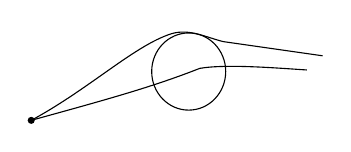
\begin{tikzpicture}[x=1cm,y=1cm]
\fill (0,0) circle (0.045);
\draw (2.0,0.62) ellipse (0.47 and 0.49);
\draw (0,0) .. controls (0.74,0.40) and (1.31,0.95) .. (1.78,1.10)
 .. controls (2.01,1.17) and (2.23,1.05) .. (2.44,1.00)
 -- (3.70,0.82);
\draw (0,0) .. controls (0.94,0.26) and (1.53,0.42) .. (2.14,0.66)
 .. controls (2.48,0.72) and (3.17,0.66) .. (3.50,0.64);
\end{tikzpicture}
\end{adjustbox}

точка и сфера: возникает 2-мерное мн-зие экстремалей

\begin{center}— $\cdot$ —\end{center}
Рассм. пр-во бинарных форм
$\left\{\sum_0^{2n-1}a_i x^i y^{2n-1-i}\right\}$ и в нём предст.
группы $SL_2(\mathbb{R})$.
[Зачёркнуто:
\Incomplete{GELFAND-P001017}{binary-cancelled-line}{Зачёркнутая фраза не поддаётся полной транскрипции; предположительные начальные фрагменты: «Это пр-во …» / «На пр-ве …». Остальной текст под перечёркиванием неразборчив}.]
При $y=1$ — просто многочл. степ. $2n-1$.

$w=\dfrac{x}{y}$ — неоднор. координата.
Запишем в ней многочлен в коорд. Дарбу:
\begin{equation*}
\frac{q_1w^{2n-1}}{(2n-1)!}+\ldots+\frac{q_nw^n}{n!}
+\frac{p_nw^{n-1}}{(n-1)!}
\Unclear{GELFAND-P001017}{polynomial-overwritten-sign}{- / + / =; исправленный знак}
\frac{p_{n-1}w^{n-2}}{(n-2)!}+\ldots+(-1)^{n-1}\frac{p_1w^0}{0!}
\end{equation*}

\SourcePage{GELFAND-P001018}{unlabelled}
% Original frame 2408 x 3496 inspected in full, including the blank lower portion.
% Text occupies approximately x390--2380,y10--1590; reading crops reviewed at 3x,
% the initially ambiguous word after p_1=1 at 5x, resolved as "условно".
% Reproducible reading crops [355,0,2350,810] and [320,820,2390,1690] at 3x;
% parenthesis [390,690,1330,815] at 3x and [1070,695,1325,810] at 5x;
% name [370,845,1110,960] at 3x; bound [395,1175,2330,1315] at 3x.
\begin{equation*}
\omega=\sum_{i=1}^{n}dp_i\wedge dq_i
\end{equation*}
Действие $SL_2(\mathbb{R})$ сохр. форму.

$w\mapsto w+t$ \underline{гамильтонов поток}; т.к. получ. из
$\begin{pmatrix}1&t\\0&1\end{pmatrix}$

Гамильтониан:
\begin{equation*}
h=q_n^2/2-q_{n-1}p_n-\ldots-q_1p_2
\end{equation*}
$q_1$ — 1-й интеграл.

Рассм. редукцию $q_1=1$ и на ней пр-во хар-к.

(берём ещё $p_1=1$ — это условно)

\underline{Вопрос И. Гольдшейда.}

Рассм. симпл. пр-во с кан. базисом $e_1,\ldots,e_n,f_1,\ldots,f_n$

Пусть $L$ — лагр. плоскость в нём. Верно ли, что сущ. (лагр.) плоскость
$L_1$, натян. на векторы $\varphi_1,\ldots,\varphi_n$, где
$\varphi_j=\alpha_j e_j+\beta_j f_j$, такая что
\begin{equation*}
\rho(L,L_1)\le 1/\sqrt{2}
\end{equation*}
(годится $<1-\varepsilon$, где $\varepsilon>0$ не зависит от размерности)

Здесь $\rho(L,L_1)=\|P_L-P_{L_1}\|$, где берётся норма (операторная) в
станд. евкл. метрике в базисе $e_1,\ldots,e_n,f_1,\ldots,f_n$.

Утверждается, что $\exists\varphi_j$ такое, что
$\sin(\widehat{\varphi_j,L})\le 1/\sqrt{2}$.

\SourcePage{GELFAND-P001019}{unlabelled}
% Direct review of original 2408 x 3496 frame. The upper region is blank.
% Review coordinates are original pixels (left,top,right,bottom), origin upper left.
% Header (200,1560,1420,2050) x3; index (100,2050,2300,2510) x3;
% lower text (100,2490,2090,3400) x2; abbreviation (225,2070,830,2155) x4;
% cancelled number (130,2150,240,2270) x10; density symbol (1530,2180,1705,2300) x8;
% coefficient sentence (1030,2400,2090,2515) x3.
% Density resolved as alpha_0 by independent comparison: P001018 alpha_j
% (1480,1110,1590,1220) x8 and P001019 (1510,2150,1665,2270) x8.
% The same left loop, ascending right stroke and short lower-right tail recur.
\underline{\underline{5/IV-82 г.}}\qquad \underline{Сем. Гельфанда.}

\underline{\underline{Водзицки}}

$M$ — мн-зие (возможно, с краем $\partial M$)

$D$ — система дифф. ур-й на $M$:
\begin{equation*}
(1)\qquad D:\ C^{\infty}(M,E)\longrightarrow C^{\infty}(M,E)
\end{equation*}
\underline{эллиптически опрд.} ($\sigma_D$ обратим).

[Перед номером (2) зачёркнуто:
\Unclear{GELFAND-P001019}{eq-two-cancel}{неразборчивый знак}.]
\begin{equation*}
(2)\qquad \operatorname{index}D=\dim\ker D-\dim\operatorname{Coker}D
=\int_M\alpha_0(x)\qquad\text{(Атья-Зингер)}
\end{equation*}
[Под $\alpha_0(x)$: \underline{плотность}.]

(2) — пример локальной формулы.

Коэфф. $\alpha_0$ выраж. через символ. Здесь естеств. появл. $\zeta$-ф-я
\begin{equation*}
(3)\qquad \zeta_A(s)=\sum_{\lambda\in\operatorname{Spec}A}\lambda^{-s}
\end{equation*}
\begin{equation*}
A=D^*D,\quad DD^*.
\end{equation*}
\begin{equation*}
z_j=\frac{n-j}{m}\text{ — полюса},\qquad n=\dim M,\quad m=\text{порядок }A.
\end{equation*}
\begin{equation*}
z_j=0,-1,-2,\ldots\quad\text{— }\underline{\text{полюсов нет.}}
\end{equation*}
\begin{equation*}
\int_M\underbrace{\zeta_A(0;x)}_{\text{плотность}}=\zeta(0);
\qquad \zeta_A(0;x)\text{ явно вычисляется}
\end{equation*}
\begin{equation*}
(4)\qquad \operatorname{index}D=\zeta_{1+D^*D}(0)-\zeta_{1+DD^*}(0)
\end{equation*}

\SourcePage{GELFAND-P001020}{unlabelled}
% Direct review of original 2408 x 3496 frame, with overlapping x2 crops covering all writing.
% Review: top (220,0,2270,780); middle (220,765,2180,1690);
% math (220,1680,2360,2420); bottom (210,2380,2408,3496).
% Enlarged details, in original pixels: coefficient (835,75,1040,205) x8;
% b symbol (1330,40,1900,240) x4; d xi prime (1050,75,1210,208) x8;
% involution (1730,1030,2295,1340) x4, resolved as plain tau by comparison
% with P001015 (1190,2840,1330,2940) x8: the detached top stroke belongs to tau.
% Kahler sentence (420,1900,1660,2100) x3;
% cancellation (653,1920,770,2055) x10; Todd text (400,2060,1980,2180) x3;
% cohomology (1410,2250,2408,2405) x3; metric (980,2520,2325,2745) x3;
% question cancellation (915,2790,1065,2865) x10;
% double (945,2860,1260,3015) x4 and seam (1050,2915,1110,2995) x10;
% final lines (405,3150,2375,3415) x3.
\begin{equation*}
(5)\qquad \zeta_A(0;x)=-\frac{1}{m}\int_{|\xi|=1}d\xi'
\int_0^{\infty}\operatorname{tr}b^{0}_{-m-n}(x,\xi,\lambda)\,d\lambda
\end{equation*}
[После знака равенства перед $-\frac{1}{m}$ зачёркнуто:
\Unclear{GELFAND-P001020}{eq-five-cancel}{неразборчивый символ или множитель}.]
\Unclear{GELFAND-P001020}{parametrix-superscript}{$b^{0}_{-m-n}$ / $b^{o}_{-m-n}$ / $b^{\circ}_{-m-n}$.}

[От $b^{0}_{-m-n}$ проведена линия к пояснению справа:]
компонента символа параметрикса $(A-\lambda)$ в нек-рой карте.

$\zeta_A(0,x)\,dx$ — это плотность (!) — не очевидно.

Пусть $\partial M\ne\varnothing$.
\Unclear{GELFAND-P001020}{upper-boundary-condition}{Условие $\partial M\ne\varnothing$ сохранено как написано.}

$D$ — опер. сигнатуры (Дирака)

Для него:
\begin{equation*}
(6)\qquad \operatorname{index}D=\operatorname{sign}M
\end{equation*}
\begin{equation*}
(7)\qquad \int_M L_k(p)=\operatorname{index}D=\int_M\alpha_0(x)
\end{equation*}
\begin{equation*}
D:\Omega_+\longrightarrow\Omega_-
\end{equation*}
$\Omega_{\pm}$ — формы, чётные (неч.) отн. инволюции
$\tau$
$=i^{np+n+1}*$ (на $p$-формах).
\begin{equation*}
(8)\qquad d+d^*=D|_{\Omega_+}:\Omega_+\longrightarrow\Omega_-.
\end{equation*}

\underline{Пример} (И.М.Г.)
\begin{equation*}
(9)\qquad
\begin{pmatrix}0&\operatorname{div}\\\operatorname{grad}&\operatorname{rot}\end{pmatrix}^{2}
=\Delta\underset{\text{ед. матр.}}{I}\qquad\text{(в }R^4\text{)}
\end{equation*}

\begin{equation*}
(10)\qquad \underline{\text{Теорема.}}\quad L_k(p)=\alpha_0(x)
\qquad\text{(Atiyah-Bott-Patodi)}
\end{equation*}
\begin{equation*}
n=4\quad\Rightarrow\quad\alpha_0(x)=\frac{1}{3}p_1
\end{equation*}

\underline{Случай}
[зачёркнуто: \Unclear{GELFAND-P001020}{kahler-cancel}{неразборчивые знаки перед $D$}]
\underline{$D=\bar{\partial}$} и $M$ — кэлерова
[над $M$ вставлено: «метрика»]
$\Rightarrow$ лок. совп. $\alpha_0(\ldots)$ и
\Unclear{GELFAND-P001020}{todd-abbreviation}{соотв. / соств.}
рода Тодда $T(p)$ (в общ. случае \underline{неверно}).

Т.е. есть 2 лок. ф-лы, к-рые не совпадают.

$\partial M\ne\varnothing\Rightarrow$ тоже есть \underline{сигнатура}
(вырожд. форма на средних когом. — нули не учит.)
\begin{equation*}
(11)\qquad
\underset{\substack{\text{топ.}\\\text{инвар.}}}{\operatorname{sign}M}
=\underbrace{\int_M L_k(p)}_{\text{лок. ф-ла}}
-\underbrace{\eta(\partial M)}_{\substack{\text{зависит}\\\text{от метрики}\\\text{на крае}}}
\end{equation*}
[К пояснению под $\eta(\partial M)$: (метр. в окр. края — \underline{произведение}).]

\underline{И.М.Г. Задача}: верно ли, что $\operatorname{sign}$ —
\underline{единств. аддитивный} инвариант для мн-зий
[зачёркнуто: \Unclear{GELFAND-P001020}{question-cancel}{неразборчивое короткое слово}]
с \underline{краем}?

Перех. на дубль:
\SourceFigure{GELFAND-P001020}{double-diagram}{Две округлые доли соединяются узкой перетяжкой; в перетяжке две дуги, правая с разрывом сверху. Справа от рисунка стоит стрелка следования. Точный характер соединения и разрывов требует сверки с оригиналом.}
$\Rightarrow$ видно по теор. Хирцебруха (рав. (7)),
что $\eta(\partial M)$ \underline{не зависит от заклейки}.

(12)\qquad $\eta(\partial M)$ — нелок. инвариант!

Локальность $\Rightarrow$ Мультиплик.
(\underline{отн.} [вставлено над строкой] перех. к накрытиям)

Есть примеры (линзовые пр-ва), когда это не так.


\SourcePage{GELFAND-P001021}{58}
% Исходный кадр 2408 x 3496 px. Координаты областей в журнале:
% начало координат — левый верхний угол; прямоугольники x0,y0,x1,y1.
% Полный оригинал просмотрен; текстовые области увеличены в 3 раза,
% отдельные знаки и зачёркивания — в 8–10 раз, рисунок на полях — в 5 раз.

(13) \underline{Теорема.} (Atiyah-Patodi-Singer)

$N=\partial M$, $D$ — элл. 1-го порядка

\begin{equation}
D=\frac{\partial}{\partial u}+A,\qquad A\text{ — опер. на }\partial M
\tag{14}
\end{equation}
(в окр. края)

Пусть $A$ \underline{нормальный} со спектром, не
[зачёркнуто: \Unclear{GELFAND-P001021}{spectrum-cancel}{сод. / соб.}]
пересек. с конич. окр. $iR$

\SourceFigure{GELFAND-P001021}{margin-spectrum}{На правом поле три пересекающиеся линии: почти вертикальная и две наклонные; в месте пересечения густой чёрный узел. Подписей не видно.}

Тогда $\exists$ эллипт. краев. условия для $D$

$P_A$ — проектор на соб. знач. $A$ с $\operatorname{Re}A\geq 0$.
\Unclear{GELFAND-P001021}{projection-real-part}{В условии написано $\operatorname{Re}A\geq 0$.}

\begin{equation}
\left\{
\begin{aligned}
Df\\
P_A(f|_A)=0
\end{aligned}
\right\}
\quad\text{— }\underline{\text{нелок. краев. задача}}
\tag{15}
\end{equation}
\Unclear{GELFAND-P001021}{boundary-restriction}{Индекс ограничения в (15) читается как $A$.}

лок. зад. сущ. не всегда.

Однако: всегда сущ. нелок.
[зачёркнуто: \Unclear{GELFAND-P001021}{nonlocal-cancel}{неразборчивый знак}]
задача!!

Тогда:
\begin{equation}
\operatorname{index}D=\int\alpha_0(x)-\frac{h_0+\eta(A)}{2},
\tag{16}
\end{equation}
где

$h_0=\dim$ [зачёркнуто:
\Unclear{GELFAND-P001021}{kernel-cancel}{$\operatorname{Ker}A$ / $\operatorname{Ker}A_0$}]
(пр-ва чисто мнимых соб. чисел).

\begin{equation}
\eta(A)\equiv\eta(0,A),\qquad
\eta(s,A)=\sum_{\lambda\in\operatorname{Spec}A}
\operatorname{sign}\operatorname{Re}\lambda\,
|\operatorname{Re}\lambda|^{-s}
\tag{17}
\end{equation}

\underline{Суть:} обобщение $L$-ф-и.

У [зачёркнуто: \Unclear{GELFAND-P001021}{attribution-cancel}{Водз. / Водз}]
A.-P.-S. \underline{$A$ — самосопр. оператор}

\underline{Теорема.} $A$ — элл. опер.

\begin{equation*}
\int_{N\times I}L_k(p)=\eta_{p_1}-\eta_{p_2}
\end{equation*}
\Unclear{GELFAND-P001021}{cylinder-formula-symbol}{Буква $p$ в формуле: $p$ / $\rho$.}

\SourceFigure{GELFAND-P001021}{cylinder-diagram}{Горизонтальный цилиндр: два узких овальных торца соединены верхней и нижней линиями. Над ним $N\times I$; под левым торцом $p_1$ или $\rho_1$, под правым $p_2$ или $\rho_2$. Стрелок не видно.}

\SourcePage{GELFAND-P001022}{unlabelled}
\underline{12/IV — 82 г.}\qquad \underline{Сем. Гельфанда.}

\underline{Водзицки.} (\underline{Мариуш})

$X$ — комп. \Unclear{GELFAND-P001022}{manifold-abbreviation}{мн-зие} с краем

(1) $D\colon C^{\infty}(X,E)\to C^{\infty}(X,F)$ эллипт. система 1-го порядка, к-рая
(дифференц.)
вблизи $\partial X$ имеет вид

\begin{equation*}
(2)\qquad D=\frac{\partial}{\partial u}+A,\qquad A\text{ — оператор на краю}
\end{equation*}

\begin{equation*}
(3)\qquad A\colon C^{\infty}(Y,E|_Y)\longrightarrow C^{\infty}(Y,F|_Y)
\end{equation*}

\SourceFigure{GELFAND-P001022}{margin-spectrum}{На правом поле: вертикальная черта с поперечными штрихами, две расходящиеся группы наклонных линий сверху и снизу; справа к верхней части рисунка направлена толстая стрелка. Участок возле острия сильно зачернён, точная геометрия этого участка неразборчива.}
здесь лишь конечн. число соб. значений оператора $A$

Краевые условия:

\begin{equation*}
(4)\qquad P_+f|_Y=0,
\end{equation*}
$P_+$ — проектор на полож. соб. \Unclear{GELFAND-P001022}{projection-cancellation}{зачёркнутый знак: неразборчиво} ф-и опер. $A$.

(5) \underline{Теорема} (Atiyah–Patody–Singer)

1974 \Unclear{GELFAND-P001022}{theorem-year-connector}{и} последователи

пусть

1) $A$ \underline{нормальна} отн. рим. метрики \underline{на краю}
\qquad $(A^*A=AA^*)$

\begin{equation*}
(6)\qquad \operatorname{index}D=\int_X\alpha_0(x)\,dx-\frac{h(A)+\eta(A)}{2}
\end{equation*}

\begin{equation*}
(7)\qquad \eta(A,s)=\sum\operatorname{sign}\operatorname{Re}\lambda\cdot
|\operatorname{Re}\lambda|^{-s},\qquad \eta(A)=\eta(A,0)
\end{equation*}

\begin{equation*}
(8)\qquad h(A)=\dim\left\{\begin{gathered}\text{мнимые}\\\text{соб. знач. }A\end{gathered}\right\}
\end{equation*}

\SourcePage{GELFAND-P001023}{64}

\underline{Док-во.} Используем ф-лу:
\begin{equation*}
(9)\qquad \operatorname{index}D=
\begin{array}[t]{c}
\operatorname{Tr}e^{-tD^{*}D}\\
\vert\vert\vert\\
\displaystyle\sum_{\lambda\in\operatorname{Spec}D^{*}D}e^{-t\lambda}
\end{array}
-
\begin{array}[t]{c}
\operatorname{Tr}e^{-tDD^{*}}\\
\Vert\\
\displaystyle\sum_{\mu\in\operatorname{Spec}DD^{*}}e^{-t\mu}
\end{array}
\end{equation*}

\SourceFigure{GELFAND-P001023}{upper-left-figure}{Вытянутый вверх, слегка наклонённый вправо замкнутый контур с подписью $e_1$; к его нижней части примыкает короткий участок с подписью $e_2$. Поперечные края изображены дугами, частью прерывистыми, напоминающими эллипсы. Справа снизу стоит знак, похожий на $Y$ или $\gamma$.}

\begin{center}— · —\end{center}

$A$ — самосопр. [Зачёркнуто: \Unclear{GELFAND-P001023}{operator-cancellation}{неразборчивое слово}.] эллипт. опер.

\begin{equation*}
(10)\qquad \sum_{\lambda>0}\lambda^{-s}=\zeta_+(s),\qquad
\zeta_+(A)\text{ — значение при }s=0.
\end{equation*}

(11) $\zeta_+(A)<\infty$, но локально имеется \underline{вычет}!!
(нелокальный ф-л)

\begin{equation*}
(12)\qquad \zeta_+(s)=\operatorname{Tr}(P_+A^{-s})
=\int_X\operatorname{Tr}(P_+A^{-s})(x,x)
\end{equation*}
[Справа: (до взятия следа были особ. при \Unclear{GELFAND-P001023}{equation-12-margin}{$s=i$ / $s=1$ / $s=0$}).]

Локальное \Unclear{GELFAND-P001023}{local-abbreviation}{слаг. / слм. / сл. / зн.} имеет вычет, и $\displaystyle\int_X$ этого вычета $=0$.

\begin{equation*}
(13)\qquad
\left\{
\begin{aligned}
\zeta(A)&=\zeta_+(A)+\zeta_-(A)\\
\eta(A)&=\zeta_+(A)-\zeta_-(A)
\end{aligned}
\right.
\end{equation*}

\underline{И. М. Г.:} в раб. Габриэлов, Гельфанд, Фукс есть алгебр. причины нелокальности.

\underline{Самая замеч. задача не сделана}: это делается для вычисл. \Unclear{GELFAND-P001023}{pontryagin-abbreviation}{знач.} на границе форм \underline{Понтрягина}, но \underline{для общих} классов ничего нет.

\begin{equation*}
\begin{array}{l|l|l}
\underline{\text{Stredder}}&\text{J. Diff. Geometry}&\text{о естеств. дифф. операторах.}\\
\underline{\text{Epstein}}&\underline{10}\ (1975),\ 645&\\
\text{(2 раб.)}&&
\end{array}
\end{equation*}

\begin{center}— · —\end{center}

\underline{Вопрос И. М. Г.:} зачем самосопряженность $A$?

Пусть дана область и на ней опр. $A$.

\begin{adjustbox}{max width=\linewidth}
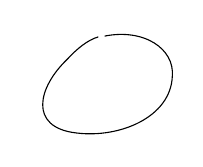
\begin{tikzpicture}[x=1cm,y=1cm]
\draw (0.84,1.30) .. controls (1.34,1.40) and (1.73,1.14) .. (1.70,0.79)
.. controls (1.68,0.27) and (1.03,0.00) .. (0.48,0.07)
.. controls (-0.13,0.14) and (-0.01,0.65) .. (0.37,1.01)
.. controls (0.48,1.13) and (0.62,1.25) .. (0.76,1.29);
\end{tikzpicture}
\end{adjustbox}

Строится теория \underline{кобордизмов}.

\underline{Инвариант} [под ним: $\eta(A)$] $A$ строится с пом. плёнки, натян. на \Unclear{GELFAND-P001023}{manifold-abbreviation}{м-зие / мн-зие}

\begin{center}— · —\end{center}

Но; в случае отсутствия заклейки не доказано!!

\begin{center}— · —\end{center}

\begin{equation*}
(14)\qquad \alpha_0(x)=\zeta(D^{*}D+\varepsilon,x)-\zeta(DD^{*}+\varepsilon,x)
\end{equation*}

\SourcePage{GELFAND-P001024}{unlabelled}

Ф-ла для $\zeta(A,x)$

\begin{equation*}
\frac{1}{m}\int_{|\xi|=1}d\xi'\int_0^\infty
b^{\Unclear{GELFAND-P001024}{formula15-superscript}{\circ}}_{-m-n}(x,\xi,\lambda)\,d\lambda
\tag{15}
\end{equation*}

[На левом поле, со стрелкой к (15) и двумя вертикальными чертами справа:]
у Сили неверный знак

\begin{center}
\begin{adjustbox}{max width=\linewidth}
\begin{tikzpicture}[x=1cm,y=1cm]
\draw[->] (0,-0.65) -- (0,2.15);
\draw[->] (0,0) -- (4.25,0);
\draw (0,0) -- (2.05,2.15);
\draw (0.65,0) arc (0:46:0.65);
\node at (0.88,0.34) {$\theta$};
\end{tikzpicture}
\end{adjustbox}
\end{center}

\begin{equation*}
\zeta_\theta(s)=\sum\lambda^{-s}
\end{equation*}
(с разрезом по лучу, идущему под углом $\theta$)

[Зачёркнуто перед формулой (16):
\Unclear{GELFAND-P001024}{formula16-cancellation}{$\zeta_\theta(s)=$}.]

\begin{equation*}
\zeta_\theta^A\bigl(\Unclear{GELFAND-P001024}{formula16-first-argument}{0\text{ или }\theta},x\bigr)
=-\frac{e^{i\theta}}{m}\int_{|\xi|=1}d\xi'\int_0^\infty
b^{\Unclear{GELFAND-P001024}{formula16-superscript}{\circ}}_{-m-n}(x,\xi,e^{i\theta}\lambda)\,d\lambda
\tag{16}
\end{equation*}
(это прав. формула)

\underline{И. М. Г.} \underline{Замеч. опер. в $\mathbb{R}^3$} (эллиптический):

\begin{equation*}
\mathcal{A}\varphi=
\begin{pmatrix}
0&\operatorname{div}\\
\operatorname{grad}&\operatorname{rot}
\end{pmatrix}
\begin{pmatrix}\varphi_0\\\vec\varphi\end{pmatrix}
=\bigl(\operatorname{div}\vec\varphi,\,
\operatorname{grad}\varphi_0+\operatorname{rot}\vec\varphi\bigr)
\tag{17}
\end{equation*}
\begin{equation*}
\mathcal{A}^2=\begin{pmatrix}\Delta&0\\0&\Delta\end{pmatrix}.
\end{equation*}
\Unclear{GELFAND-P001024}{operator17-square}{Знаки в записанном равенстве для $\mathcal{A}^2$ сохранены.}

\begin{center}
\begin{adjustbox}{max width=\linewidth}
\begin{tikzpicture}[x=1cm,y=1cm]
\draw (0,0) -- (0.4,-0.02);
\fill (0.65,-0.01) circle (0.015);
\draw (0.87,0) -- (1.5,0);
\end{tikzpicture}
\end{adjustbox}
\end{center}

$A$ --- элл. опер. на замкн. мн-зии, спектр $A$ не
\Unclear{GELFAND-P001024}{spectrum-word}{заполняет / зацепляет}
сектора ок. луча (луч. $\min$ роста)

\begin{center}
\begin{adjustbox}{max width=\linewidth}
\begin{tikzpicture}[x=1cm,y=1cm]
\node[anchor=west] at (0.6,1.5) {$\zeta_{\theta,A}(s)=\sum\lambda_\theta^{-s}$};
\draw (0.55,1.24) -- (0.55,1.05) -- (4.9,1.05) -- (4.9,1.24);
\draw (0.1,0.5) -- (0.82,0.84);
\draw (0.1,0.5) -- (0.79,-0.22);
\node at (1.05,0.9) {$\theta$};
\node at (1.03,-0.34) {$\theta'$};
\end{tikzpicture}
\end{adjustbox}
\end{center}
\underline{по лучу определим.}

Пусть $\theta'$ --- другой луч $\min$ роста.

\begin{equation*}
\zeta_{\theta',A}(s)=\sum\lambda_{\theta'}^{-s}
\end{equation*}
$\Rightarrow$ спектр в 2-х секторах

\SourceFigure{GELFAND-P001024}{spectral-sectors-diagram}{Слева округлый контур с разрывом сверху и подписью $D''$ выше слева; справа вытянутый округлый контур с $D'$ внутри. Между ними почти вертикальная линия и два наклонных луча из общей точки вправо вверх и вправо вниз; в общей точке маленькая петля. Возле нижнего конца наклонного луча короткая засечка. Замкнутость левого контура и наличие стрелки у нижнего луча не установлены.}

(18) \underline{Теорема}.
\begin{equation*}
\rho(s)\overset{\mathrm{def}}{=}\zeta_\theta(A,s)-\zeta_{\theta'}(A,s)
\end{equation*}
Тогда

а) $\rho(s)$ мероморфна с вычетами в
$z_j=\dfrac{-j+n}{m}$, $j=0,1,2,\ldots$

б) $z_j\in\mathbb{Z}\Rightarrow$ вычет исчезает микролокально!!

(элементарно!)

\SourcePage{GELFAND-P001025}{65}
% Исходный кадр 2408 x 3496 px. Координаты областей в журнале:
% начало координат — левый верхний угол; прямоугольники x0,y0,x1,y1.

в)
\begin{equation*}
\begin{array}[t]{c}z_j\\\Vert\\\ell\end{array}
\in\mathbb{Z}\Rightarrow
\begin{array}[t]{c}\rho(z_j)\\\Vert\\\rho(\ell)\end{array}
\text{ зад. }\underline{\text{локальными ф-иями}}
\end{equation*}
(содержат. утвержд., — верно и для п. д. о.!)

\begin{equation*}
(19)\qquad
\rho(i)\overset{\mathrm{def}}{=}\int_X\rho_i(x)\,dx
=-\frac{2\pi i}{m}\int_X dx\int_{|\xi|=1}d\xi'
\sum_{\lambda_\nu\in D'}\operatorname{Res}
\frac{\operatorname{tr}b^{\Unclear{GELFAND-P001025}{formula19-b-superscript}{\circ}}_{m(i-1)-n}(x,\xi,\lambda)}{\lambda^i}
\end{equation*}
\Unclear{GELFAND-P001025}{formula19-integer-symbol}{В (19) знак в аргументе $\rho$, индексе $\rho$, индексе $b$ и показателе $\lambda$: $i$ / $\ell$.}

г) $\ell\in\mathbb{Z}_-=\{0,-1,-2,-3,-4,\ldots\}\Rightarrow\rho(\ell)=0$

(усил. версия A.-P.-S.).

\underline{Подсказки} (к г)):

Надо док. не про \Unclear{GELFAND-P001025}{hint-word}{вычеты / исчезн.} в $0$, а про все целые точки $>0$
\Unclear{GELFAND-P001025}{hint-integer-range}{В подсказке написано $>0$.}

В точке $0$ получается: надо использовать преобр. Малера (из $p$-адич. чисел):

\begin{equation*}
(20)\qquad
\zeta_\theta(-k,A+t)
=\sum_{\nu=0}^{k}\binom{k}{\nu}\zeta(\nu-k,A)t^\nu
+t^k\sum_{\mu=1}^{n}
\frac{(-1)^\mu\delta_\mu}{\binom{\mu+k}{k}\mu}
\end{equation*}
[Под первой суммой:] \underline{\underline{полином:}}
\Unclear{GELFAND-P001025}{formula20-second-sum}{Второй член (20) записан с $t^k$ перед суммой; дополнительной степени $t$ в её слагаемом не видно.}

$\delta_\mu$ — вычет в точке $\mu$ для $\zeta$-ф-и оператора $A$

Это для опер. 1-го порядка.

\begin{equation*}
\operatorname{Ker}A\ne\{0\}\Rightarrow
\text{вместо }\zeta(0)\text{ надо написать }
\zeta(0)+h_0(A)
\end{equation*}
[Под $\zeta(0)+h_0(A)$ — прямая нижняя скобка с короткими вертикальными штрихами на концах.]
$(h_0(A)=\dim\operatorname{Ker}A).$

[Зачёркнуто: \Unclear{GELFAND-P001025}{mahler-cancellation}{Теор. / неразборчивое слово}.]
1-я сумма в (20) — \underline{пр. Малера.}

Автоморфная ф-я отн. преобр. Малера продолж. в $p$-адич. область.



\end{document}
